\documentclass[]{article}
\usepackage{lmodern}
\usepackage{amssymb,amsmath}
\usepackage{ifxetex,ifluatex}
\usepackage{fixltx2e} % provides \textsubscript
\ifnum 0\ifxetex 1\fi\ifluatex 1\fi=0 % if pdftex
  \usepackage[T1]{fontenc}
  \usepackage[utf8]{inputenc}
\else % if luatex or xelatex
  \ifxetex
    \usepackage{mathspec}
  \else
    \usepackage{fontspec}
  \fi
  \defaultfontfeatures{Ligatures=TeX,Scale=MatchLowercase}
\fi
% use upquote if available, for straight quotes in verbatim environments
\IfFileExists{upquote.sty}{\usepackage{upquote}}{}
% use microtype if available
\IfFileExists{microtype.sty}{%
\usepackage{microtype}
\UseMicrotypeSet[protrusion]{basicmath} % disable protrusion for tt fonts
}{}
\usepackage[margin=1in]{geometry}
\usepackage{hyperref}
\hypersetup{unicode=true,
            pdftitle={hw6},
            pdfauthor={LuchaoQi},
            pdfborder={0 0 0},
            breaklinks=true}
\urlstyle{same}  % don't use monospace font for urls
\usepackage{color}
\usepackage{fancyvrb}
\newcommand{\VerbBar}{|}
\newcommand{\VERB}{\Verb[commandchars=\\\{\}]}
\DefineVerbatimEnvironment{Highlighting}{Verbatim}{commandchars=\\\{\}}
% Add ',fontsize=\small' for more characters per line
\usepackage{framed}
\definecolor{shadecolor}{RGB}{248,248,248}
\newenvironment{Shaded}{\begin{snugshade}}{\end{snugshade}}
\newcommand{\KeywordTok}[1]{\textcolor[rgb]{0.13,0.29,0.53}{\textbf{#1}}}
\newcommand{\DataTypeTok}[1]{\textcolor[rgb]{0.13,0.29,0.53}{#1}}
\newcommand{\DecValTok}[1]{\textcolor[rgb]{0.00,0.00,0.81}{#1}}
\newcommand{\BaseNTok}[1]{\textcolor[rgb]{0.00,0.00,0.81}{#1}}
\newcommand{\FloatTok}[1]{\textcolor[rgb]{0.00,0.00,0.81}{#1}}
\newcommand{\ConstantTok}[1]{\textcolor[rgb]{0.00,0.00,0.00}{#1}}
\newcommand{\CharTok}[1]{\textcolor[rgb]{0.31,0.60,0.02}{#1}}
\newcommand{\SpecialCharTok}[1]{\textcolor[rgb]{0.00,0.00,0.00}{#1}}
\newcommand{\StringTok}[1]{\textcolor[rgb]{0.31,0.60,0.02}{#1}}
\newcommand{\VerbatimStringTok}[1]{\textcolor[rgb]{0.31,0.60,0.02}{#1}}
\newcommand{\SpecialStringTok}[1]{\textcolor[rgb]{0.31,0.60,0.02}{#1}}
\newcommand{\ImportTok}[1]{#1}
\newcommand{\CommentTok}[1]{\textcolor[rgb]{0.56,0.35,0.01}{\textit{#1}}}
\newcommand{\DocumentationTok}[1]{\textcolor[rgb]{0.56,0.35,0.01}{\textbf{\textit{#1}}}}
\newcommand{\AnnotationTok}[1]{\textcolor[rgb]{0.56,0.35,0.01}{\textbf{\textit{#1}}}}
\newcommand{\CommentVarTok}[1]{\textcolor[rgb]{0.56,0.35,0.01}{\textbf{\textit{#1}}}}
\newcommand{\OtherTok}[1]{\textcolor[rgb]{0.56,0.35,0.01}{#1}}
\newcommand{\FunctionTok}[1]{\textcolor[rgb]{0.00,0.00,0.00}{#1}}
\newcommand{\VariableTok}[1]{\textcolor[rgb]{0.00,0.00,0.00}{#1}}
\newcommand{\ControlFlowTok}[1]{\textcolor[rgb]{0.13,0.29,0.53}{\textbf{#1}}}
\newcommand{\OperatorTok}[1]{\textcolor[rgb]{0.81,0.36,0.00}{\textbf{#1}}}
\newcommand{\BuiltInTok}[1]{#1}
\newcommand{\ExtensionTok}[1]{#1}
\newcommand{\PreprocessorTok}[1]{\textcolor[rgb]{0.56,0.35,0.01}{\textit{#1}}}
\newcommand{\AttributeTok}[1]{\textcolor[rgb]{0.77,0.63,0.00}{#1}}
\newcommand{\RegionMarkerTok}[1]{#1}
\newcommand{\InformationTok}[1]{\textcolor[rgb]{0.56,0.35,0.01}{\textbf{\textit{#1}}}}
\newcommand{\WarningTok}[1]{\textcolor[rgb]{0.56,0.35,0.01}{\textbf{\textit{#1}}}}
\newcommand{\AlertTok}[1]{\textcolor[rgb]{0.94,0.16,0.16}{#1}}
\newcommand{\ErrorTok}[1]{\textcolor[rgb]{0.64,0.00,0.00}{\textbf{#1}}}
\newcommand{\NormalTok}[1]{#1}
\usepackage{graphicx,grffile}
\makeatletter
\def\maxwidth{\ifdim\Gin@nat@width>\linewidth\linewidth\else\Gin@nat@width\fi}
\def\maxheight{\ifdim\Gin@nat@height>\textheight\textheight\else\Gin@nat@height\fi}
\makeatother
% Scale images if necessary, so that they will not overflow the page
% margins by default, and it is still possible to overwrite the defaults
% using explicit options in \includegraphics[width, height, ...]{}
\setkeys{Gin}{width=\maxwidth,height=\maxheight,keepaspectratio}
\IfFileExists{parskip.sty}{%
\usepackage{parskip}
}{% else
\setlength{\parindent}{0pt}
\setlength{\parskip}{6pt plus 2pt minus 1pt}
}
\setlength{\emergencystretch}{3em}  % prevent overfull lines
\providecommand{\tightlist}{%
  \setlength{\itemsep}{0pt}\setlength{\parskip}{0pt}}
\setcounter{secnumdepth}{0}
% Redefines (sub)paragraphs to behave more like sections
\ifx\paragraph\undefined\else
\let\oldparagraph\paragraph
\renewcommand{\paragraph}[1]{\oldparagraph{#1}\mbox{}}
\fi
\ifx\subparagraph\undefined\else
\let\oldsubparagraph\subparagraph
\renewcommand{\subparagraph}[1]{\oldsubparagraph{#1}\mbox{}}
\fi

%%% Use protect on footnotes to avoid problems with footnotes in titles
\let\rmarkdownfootnote\footnote%
\def\footnote{\protect\rmarkdownfootnote}

%%% Change title format to be more compact
\usepackage{titling}

% Create subtitle command for use in maketitle
\newcommand{\subtitle}[1]{
  \posttitle{
    \begin{center}\large#1\end{center}
    }
}

\setlength{\droptitle}{-2em}

  \title{hw6}
    \pretitle{\vspace{\droptitle}\centering\huge}
  \posttitle{\par}
    \author{LuchaoQi}
    \preauthor{\centering\large\emph}
  \postauthor{\par}
      \predate{\centering\large\emph}
  \postdate{\par}
    \date{November 27, 2018}


\begin{document}
\maketitle

\subsubsection{Problem 1}\label{problem-1}

We have table shown below:\\
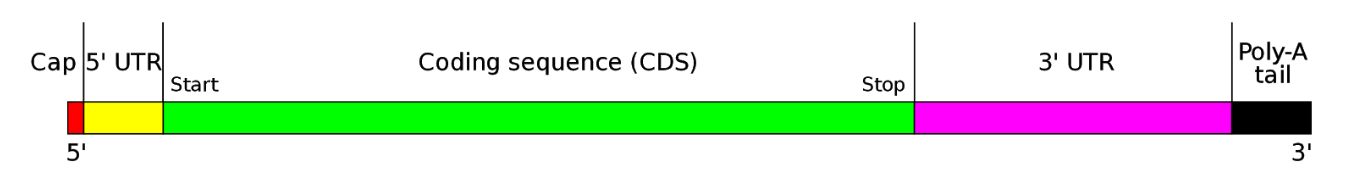
\includegraphics{C:/Users/lcqi/OneDrive/Desktop/1.png} The square of Z
statistic is: 
\includegraphics{C:/Users/lcqi/OneDrive/Desktop/2.png}
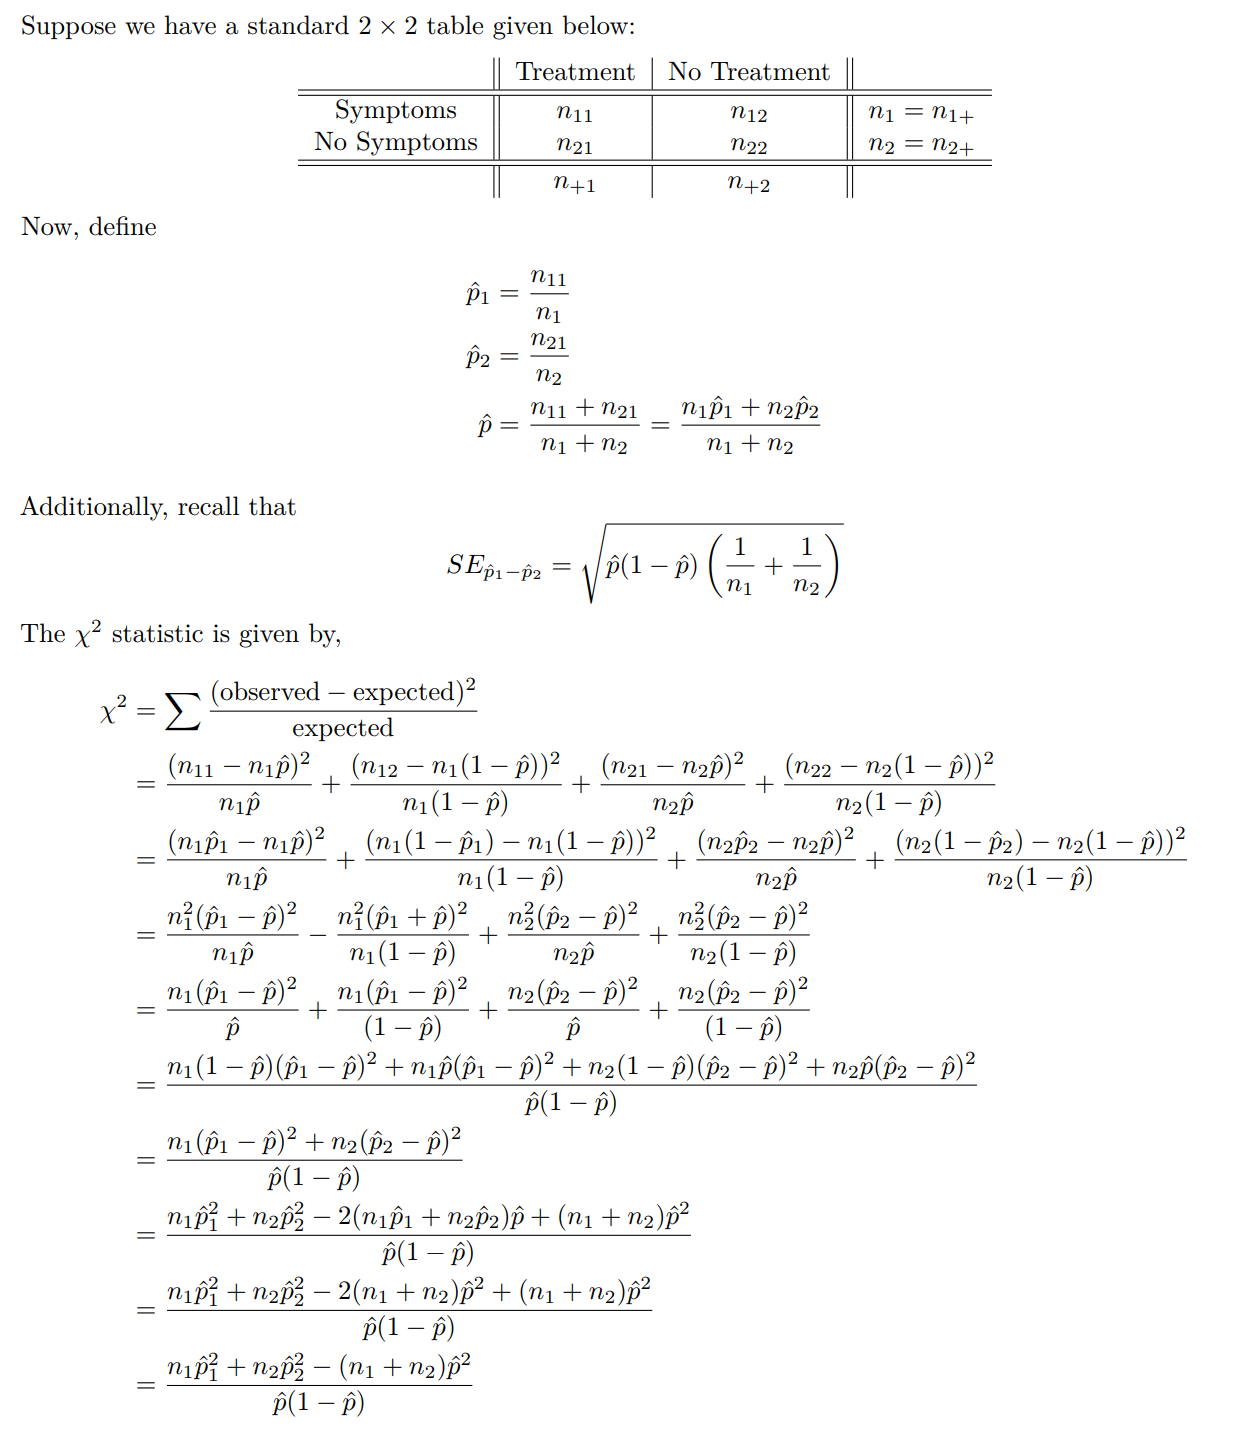
\includegraphics{C:/Users/lcqi/OneDrive/Desktop/3.png} The \(\chi^2\)
statistic is: 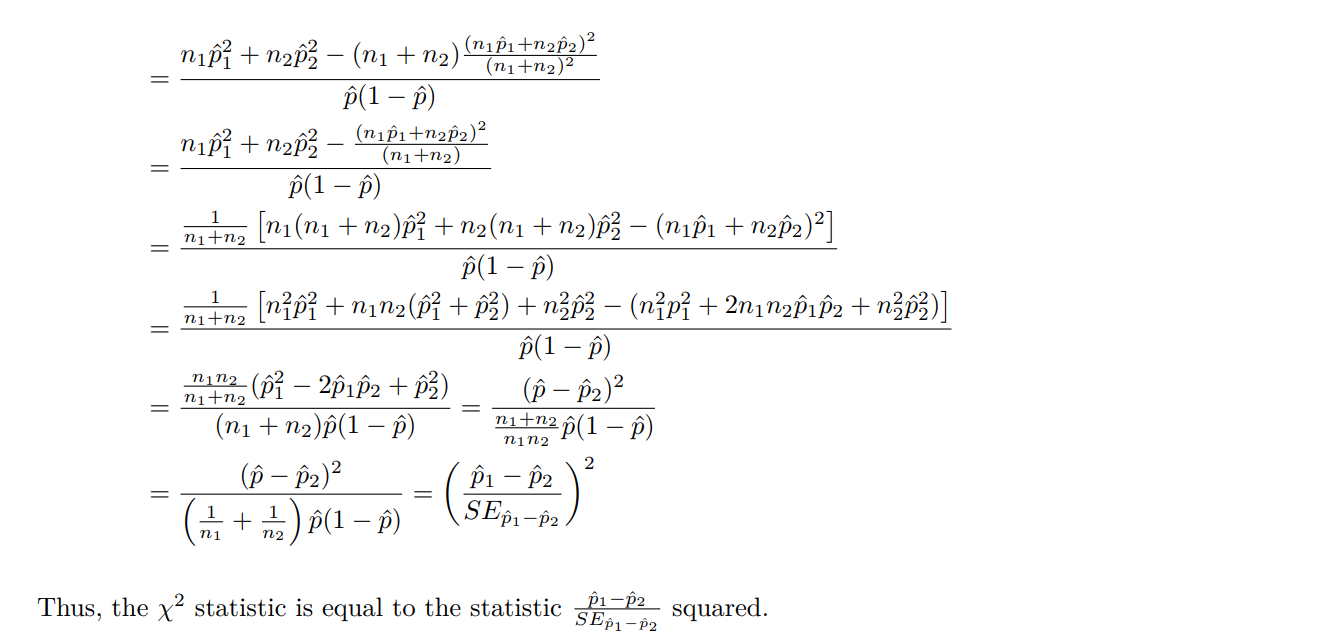
\includegraphics{C:/Users/lcqi/OneDrive/Desktop/4.png} So
we have: 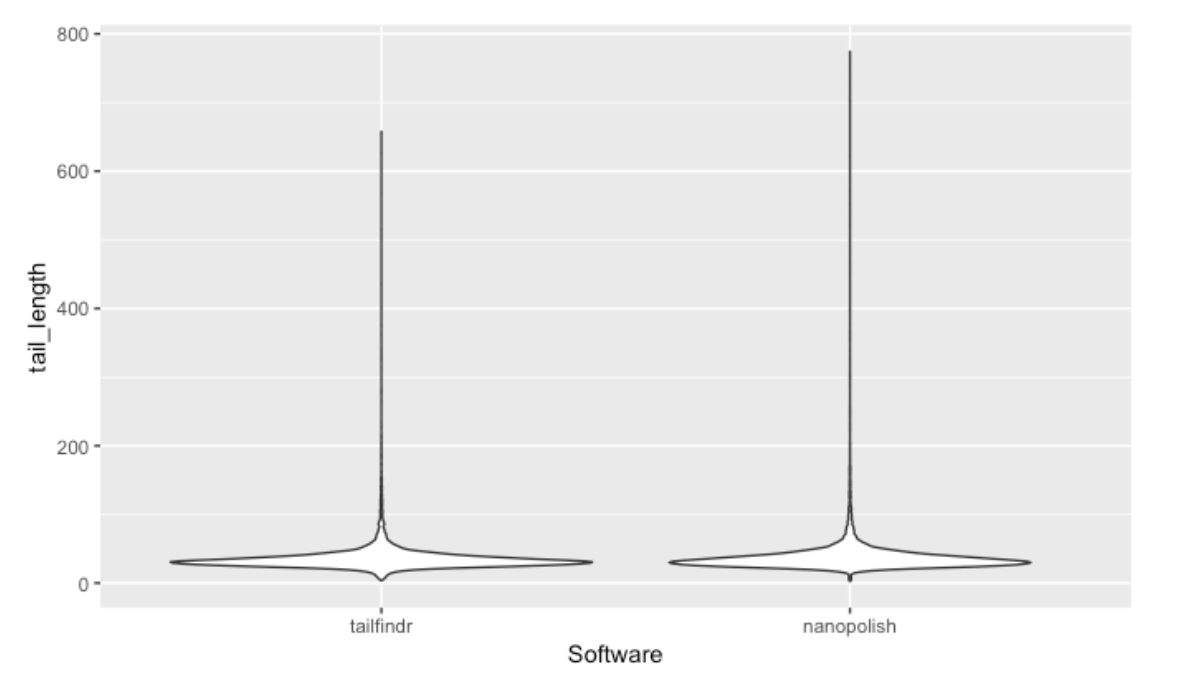
\includegraphics{C:/Users/lcqi/OneDrive/Desktop/5.png}

\subsubsection{Problem 2}\label{problem-2}

\begin{enumerate}
\def\labelenumi{\alph{enumi}.}
\tightlist
\item
  Null: \(H_0 : \hat{RD} = \hat{p1} - \hat{p2} = 0\)\\
  Alternative: \(H_A : \hat{p1} - \hat{p2} \neq0\)\\
  \({\hat{SE}}_{\hat{RD}}=\sqrt{\frac{\hat{p1}(1-\hat{p1})}{n_1}+\frac{\hat{p2}(1-\hat{p2})}{n_2}}\)
\end{enumerate}

\begin{Shaded}
\begin{Highlighting}[]
\NormalTok{x=}\DecValTok{2}\OperatorTok{/}\DecValTok{15}
\NormalTok{y=}\DecValTok{4}\OperatorTok{/}\DecValTok{19}
\NormalTok{p=}\DecValTok{60}\OperatorTok{/}\DecValTok{340}
\NormalTok{z=(y}\OperatorTok{-}\NormalTok{x)}\OperatorTok{/}\KeywordTok{sqrt}\NormalTok{(p}\OperatorTok{*}\NormalTok{(}\DecValTok{1}\OperatorTok{-}\NormalTok{p)}\OperatorTok{*}\NormalTok{(}\DecValTok{1}\OperatorTok{/}\DecValTok{150}\OperatorTok{+}\DecValTok{1}\OperatorTok{/}\DecValTok{190}\NormalTok{))}
\DecValTok{2}\OperatorTok{*}\NormalTok{(}\DecValTok{1}\OperatorTok{-}\KeywordTok{pnorm}\NormalTok{(z))}
\end{Highlighting}
\end{Shaded}

\begin{verbatim}
## [1] 0.06375422
\end{verbatim}

We could see p-value = 0.06375422\textless{}0.05, so we reject null and
conclude that the two proportions are not equal.\\
b.\\
For absolute change:\\
\(H_0 : \hat{RD} = \hat{p1} - \hat{p2} = 0\)\\
\(H_A : \hat{p1} - \hat{p2} \neq0\)\\
CI ={[}-0.155191935 0.004424391{]}

\begin{Shaded}
\begin{Highlighting}[]
\NormalTok{x=}\DecValTok{21}\OperatorTok{/}\DecValTok{152}
\NormalTok{y=}\DecValTok{41}\OperatorTok{/}\DecValTok{192}
\NormalTok{(x}\OperatorTok{-}\NormalTok{y)}\OperatorTok{+}\KeywordTok{c}\NormalTok{(}\OperatorTok{-}\DecValTok{1}\NormalTok{,}\DecValTok{1}\NormalTok{)}\OperatorTok{*}\KeywordTok{qnorm}\NormalTok{(}\FloatTok{0.975}\NormalTok{)}\OperatorTok{*}\KeywordTok{sqrt}\NormalTok{(x}\OperatorTok{*}\NormalTok{(}\DecValTok{1}\OperatorTok{-}\NormalTok{x)}\OperatorTok{/}\DecValTok{152}\OperatorTok{+}\NormalTok{y}\OperatorTok{*}\NormalTok{(}\DecValTok{1}\OperatorTok{-}\NormalTok{y)}\OperatorTok{/}\DecValTok{192}\NormalTok{)}
\end{Highlighting}
\end{Shaded}

\begin{verbatim}
## [1] -0.155191935  0.004424391
\end{verbatim}

For relative risk: we use log-transformation\\
\(H_0 : log(\hat{RR}) = log(\frac{\hat{p1}}{\hat{p2}}) = 0\)\\
\(H_A : log(\hat{RR}) = log(\frac{\hat{p1}}{\hat{p2}}) \neq 0\)\\
Interval for logRR = {[}-2.416758 1.503242{]}\\
Exponentiate it and we got CI = {[}0.3871324 1.0361082{]}

\begin{Shaded}
\begin{Highlighting}[]
\NormalTok{x=}\DecValTok{20}\OperatorTok{/}\DecValTok{150}
\NormalTok{y=}\DecValTok{40}\OperatorTok{/}\DecValTok{190}
\NormalTok{se=}\KeywordTok{sqrt}\NormalTok{((}\DecValTok{1}\OperatorTok{-}\NormalTok{x)}\OperatorTok{/}\NormalTok{(x}\OperatorTok{*}\DecValTok{150}\NormalTok{)}\OperatorTok{+}\NormalTok{(}\DecValTok{1}\OperatorTok{-}\NormalTok{y)}\OperatorTok{/}\NormalTok{(y}\OperatorTok{*}\DecValTok{190}\NormalTok{))}
\NormalTok{log=}\KeywordTok{log}\NormalTok{(x}\OperatorTok{/}\NormalTok{y)}\OperatorTok{+}\KeywordTok{c}\NormalTok{(}\OperatorTok{-}\DecValTok{1}\NormalTok{,}\DecValTok{1}\NormalTok{)}\OperatorTok{*}\FloatTok{1.96}\OperatorTok{*}\NormalTok{se}
\KeywordTok{exp}\NormalTok{(log)}
\end{Highlighting}
\end{Shaded}

\begin{verbatim}
## [1] 0.3871324 1.0361082
\end{verbatim}

For odds ratio:\\
CI = {[}0.3211208 1.0364953{]}

\begin{Shaded}
\begin{Highlighting}[]
\NormalTok{n11=}\DecValTok{20}
\NormalTok{n12=}\DecValTok{130}
\NormalTok{n21=}\DecValTok{40}
\NormalTok{n22=}\DecValTok{150}
\NormalTok{n=(n11}\OperatorTok{*}\NormalTok{n22)}\OperatorTok{/}\NormalTok{(n12}\OperatorTok{*}\NormalTok{n21)}
\NormalTok{se=}\KeywordTok{sqrt}\NormalTok{(}\DecValTok{1}\OperatorTok{/}\NormalTok{n11}\OperatorTok{+}\DecValTok{1}\OperatorTok{/}\NormalTok{n12}\OperatorTok{+}\DecValTok{1}\OperatorTok{/}\NormalTok{n21}\OperatorTok{+}\DecValTok{1}\OperatorTok{/}\NormalTok{n22)}
\NormalTok{log=}\KeywordTok{log}\NormalTok{(n)}\OperatorTok{+}\KeywordTok{c}\NormalTok{(}\OperatorTok{-}\DecValTok{1}\NormalTok{,}\DecValTok{1}\NormalTok{)}\OperatorTok{*}\NormalTok{se}\OperatorTok{*}\KeywordTok{qnorm}\NormalTok{(}\FloatTok{0.975}\NormalTok{)}
\KeywordTok{exp}\NormalTok{(log)}
\end{Highlighting}
\end{Shaded}

\begin{verbatim}
## [1] 0.3211208 1.0364953
\end{verbatim}

\begin{enumerate}
\def\labelenumi{\alph{enumi}.}
\setcounter{enumi}{2}
\item
\end{enumerate}

Bayesian credible intervals:

\begin{Shaded}
\begin{Highlighting}[]
\NormalTok{x1 =}\StringTok{ }\DecValTok{20}\NormalTok{; n1 =}\StringTok{ }\DecValTok{150}
\NormalTok{x2 =}\StringTok{ }\DecValTok{40}\NormalTok{; n2 =}\StringTok{ }\DecValTok{190}
\NormalTok{alpha1 =}\StringTok{ }\DecValTok{1}\NormalTok{; beta1 =}\StringTok{ }\DecValTok{1}
\NormalTok{alpha2 =}\StringTok{ }\DecValTok{1}\NormalTok{; beta2 =}\StringTok{ }\DecValTok{1}
\NormalTok{p1 =}\StringTok{ }\KeywordTok{rbeta}\NormalTok{(}\DecValTok{1000}\NormalTok{,x1}\OperatorTok{+}\NormalTok{alpha1, n1}\OperatorTok{-}\NormalTok{x1}\OperatorTok{+}\NormalTok{beta1)}
\NormalTok{p2 =}\StringTok{ }\KeywordTok{rbeta}\NormalTok{(}\DecValTok{1000}\NormalTok{,x2}\OperatorTok{+}\NormalTok{alpha2, n2}\OperatorTok{-}\NormalTok{x2}\OperatorTok{+}\NormalTok{beta2)}
\end{Highlighting}
\end{Shaded}

For RD:

\begin{Shaded}
\begin{Highlighting}[]
\NormalTok{rd =}\StringTok{ }\NormalTok{p1}\OperatorTok{-}\NormalTok{p2}
\KeywordTok{quantile}\NormalTok{(rd,}\KeywordTok{c}\NormalTok{(.}\DecValTok{025}\NormalTok{,.}\DecValTok{975}\NormalTok{))}
\end{Highlighting}
\end{Shaded}

\begin{verbatim}
##         2.5%        97.5% 
## -0.154242992  0.003780869
\end{verbatim}

\begin{Shaded}
\begin{Highlighting}[]
\KeywordTok{plot}\NormalTok{(}\KeywordTok{density}\NormalTok{(rd))}
\end{Highlighting}
\end{Shaded}

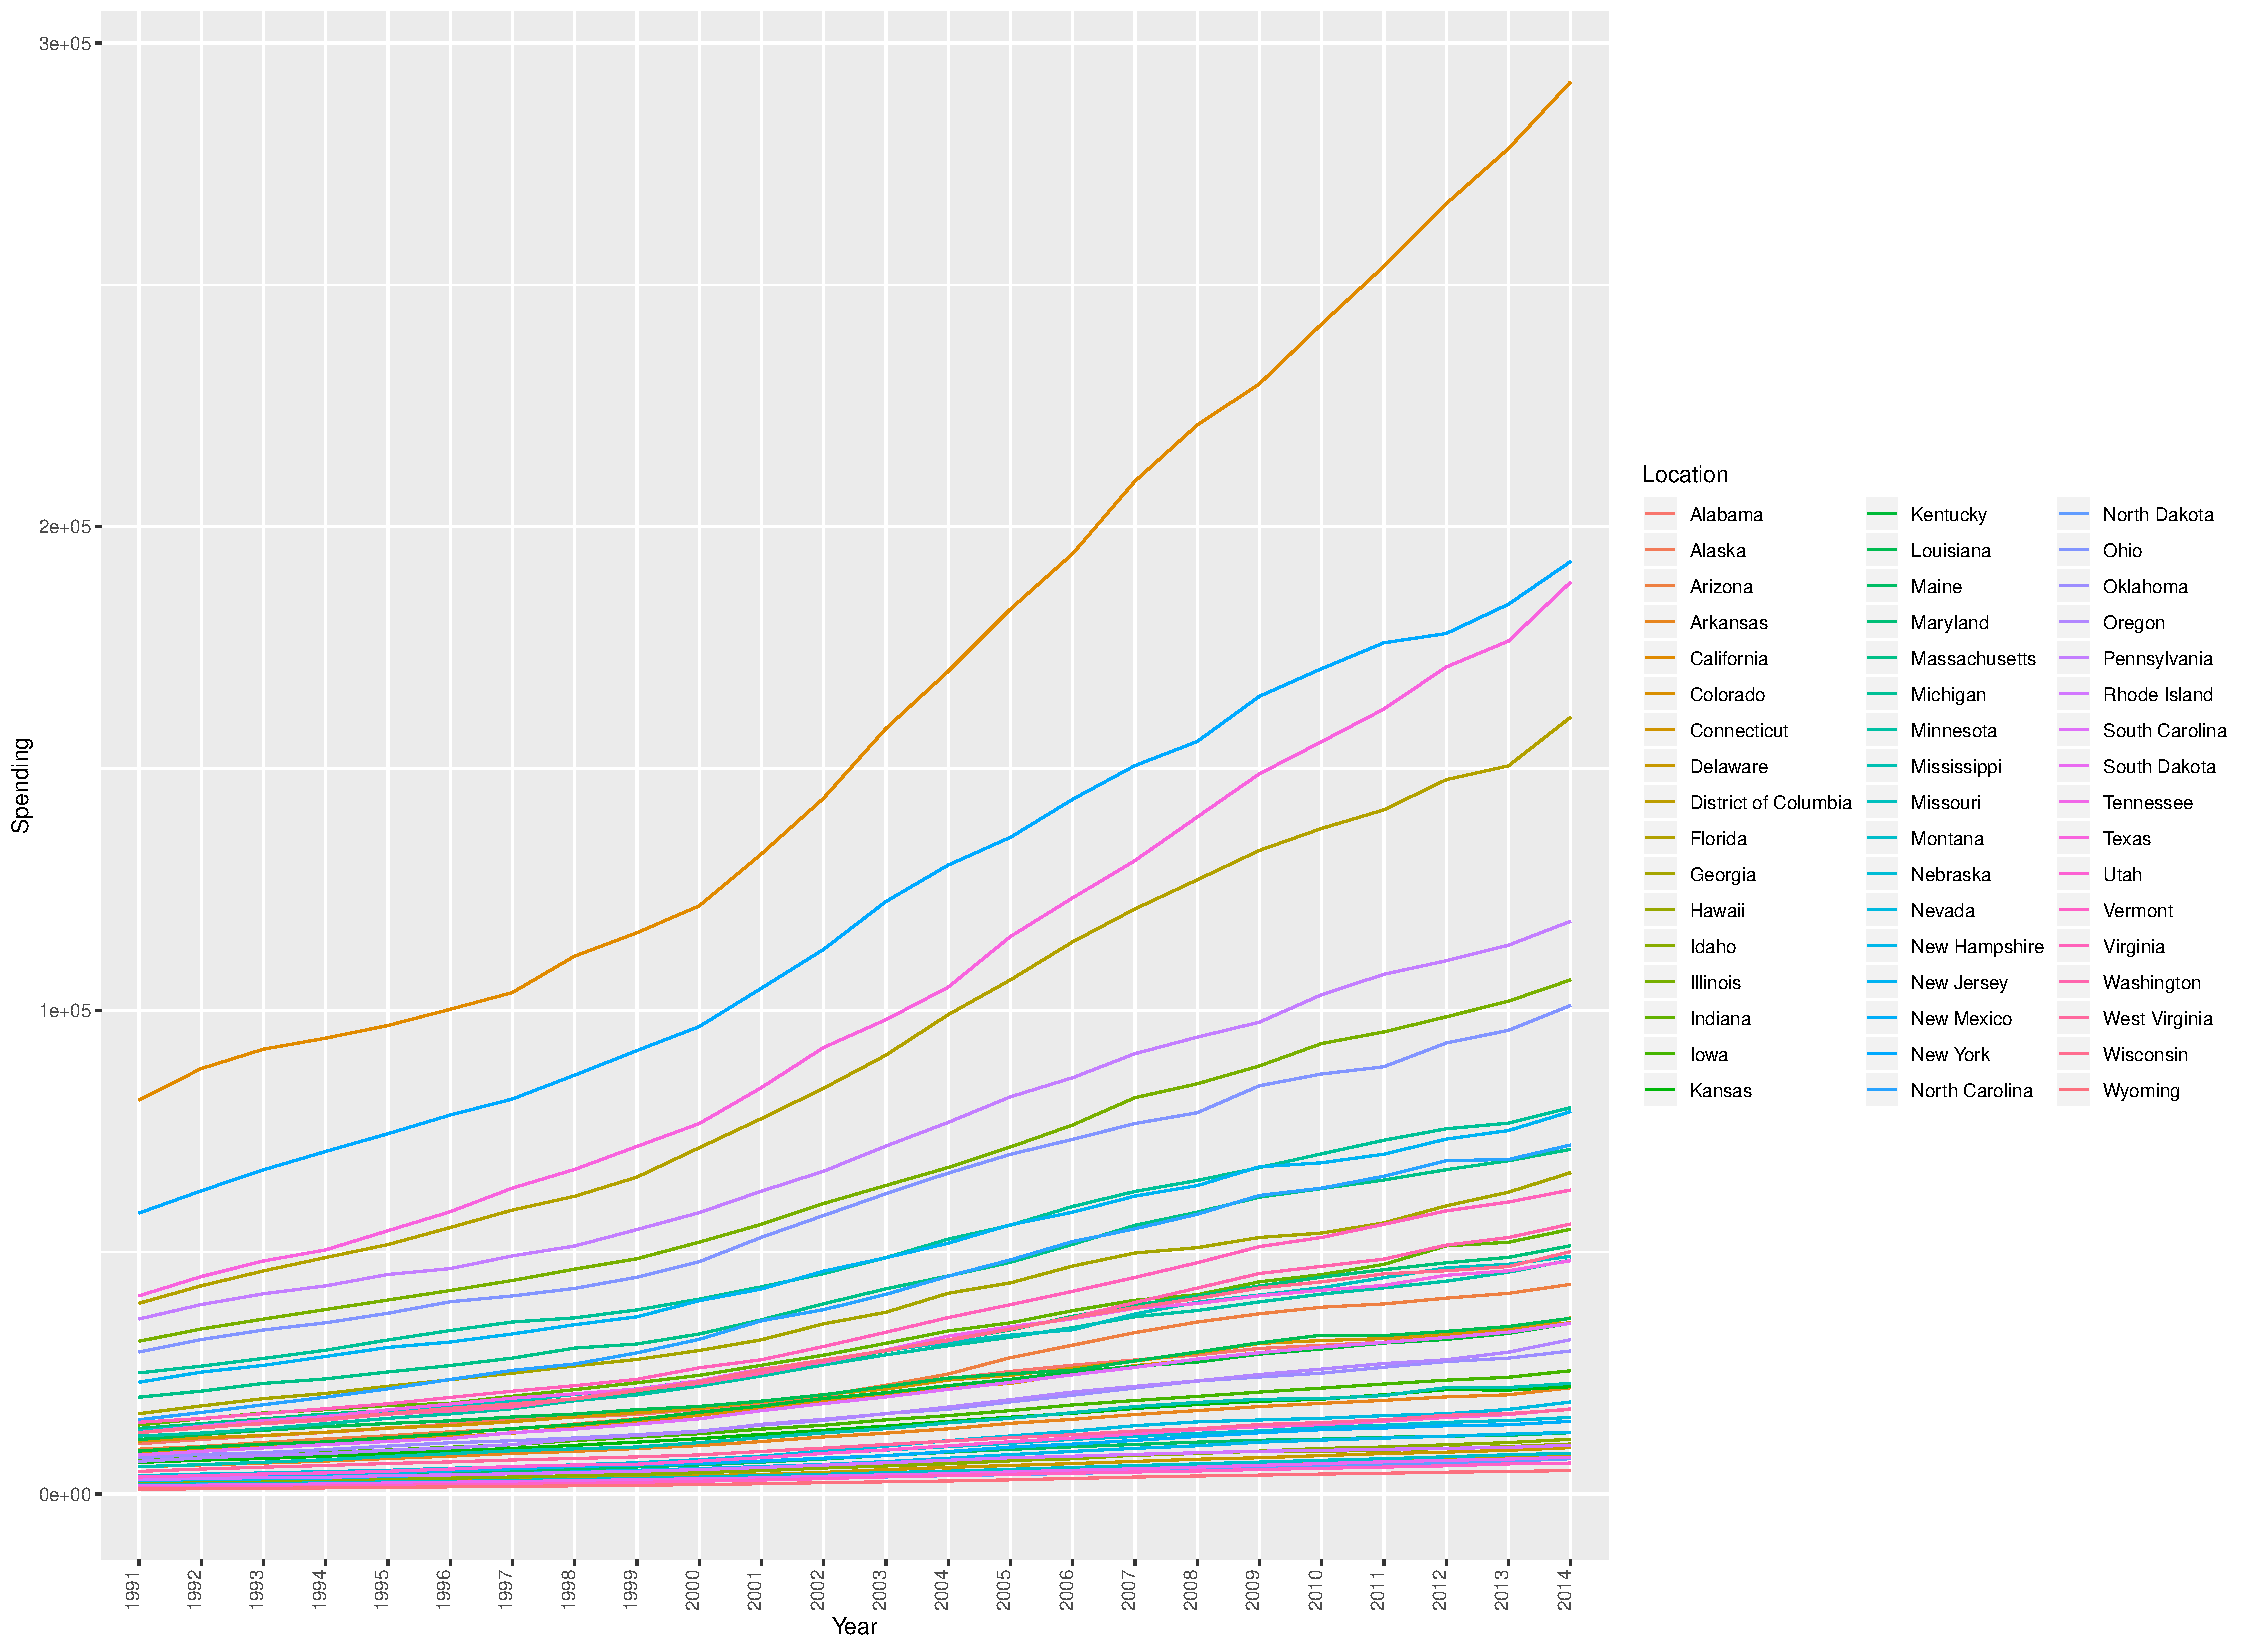
\includegraphics{hw6_files/figure-latex/unnamed-chunk-6-1.pdf} For RR:

\begin{Shaded}
\begin{Highlighting}[]
\NormalTok{rr =}\StringTok{ }\NormalTok{p1}\OperatorTok{/}\NormalTok{p2}
\KeywordTok{quantile}\NormalTok{(rr,}\KeywordTok{c}\NormalTok{(}\FloatTok{0.025}\NormalTok{,}\FloatTok{0.975}\NormalTok{))}
\end{Highlighting}
\end{Shaded}

\begin{verbatim}
##     2.5%    97.5% 
## 0.393639 1.021176
\end{verbatim}

\begin{Shaded}
\begin{Highlighting}[]
\KeywordTok{plot}\NormalTok{(}\KeywordTok{density}\NormalTok{(rr))}
\end{Highlighting}
\end{Shaded}

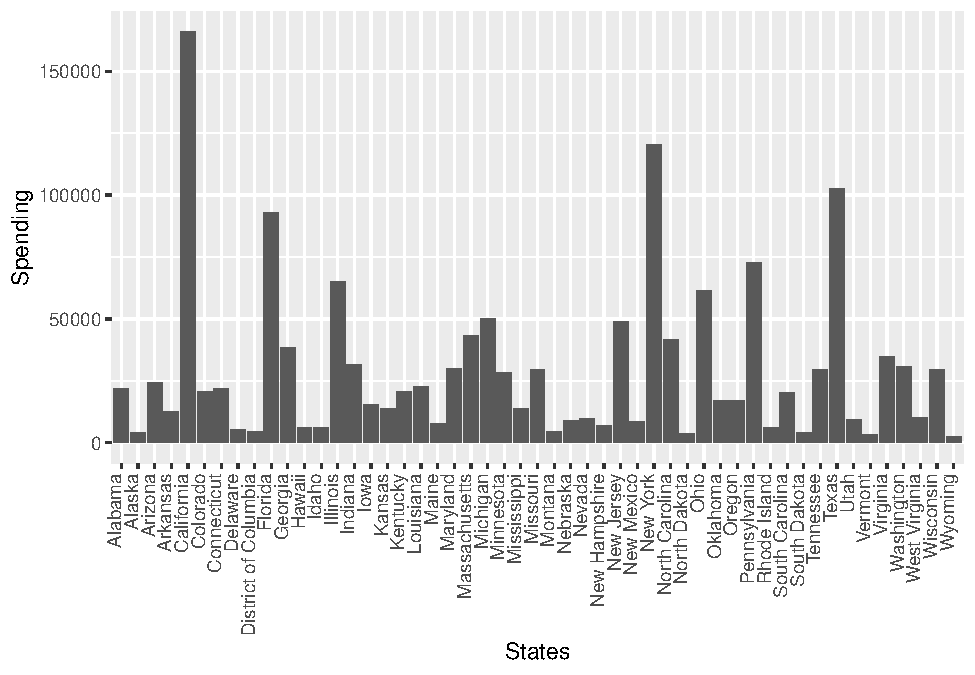
\includegraphics{hw6_files/figure-latex/unnamed-chunk-7-1.pdf} For OR:

\begin{Shaded}
\begin{Highlighting}[]
\NormalTok{or =}\StringTok{ }\NormalTok{p1}\OperatorTok{/}\NormalTok{(}\DecValTok{1}\OperatorTok{-}\NormalTok{p1)}\OperatorTok{/}\NormalTok{(p2}\OperatorTok{/}\NormalTok{(}\DecValTok{1}\OperatorTok{-}\NormalTok{p2))}
\KeywordTok{quantile}\NormalTok{(or,}\KeywordTok{c}\NormalTok{(}\FloatTok{0.025}\NormalTok{,}\FloatTok{0.975}\NormalTok{))}
\end{Highlighting}
\end{Shaded}

\begin{verbatim}
##      2.5%     97.5% 
## 0.3318204 1.0258979
\end{verbatim}

\begin{Shaded}
\begin{Highlighting}[]
\KeywordTok{plot}\NormalTok{(}\KeywordTok{density}\NormalTok{(or))}
\end{Highlighting}
\end{Shaded}

\includegraphics{hw6_files/figure-latex/unnamed-chunk-8-1.pdf}

\subsubsection{Problem 3}\label{problem-3}

95\% CI =\\
\[[log(\frac{x}{n})-1.96*\sqrt{\frac{1}{x}-\frac{1}{n}},log(\frac{x}{n})+1.96*\sqrt{\frac{1}{x}-\frac{1}{n}}]\]

\subsubsection{problem 4}\label{problem-4}

\begin{enumerate}
\def\labelenumi{\alph{enumi}.}
\tightlist
\item
  \({\frac{\hat{p}-p}{\hat{SE}_\hat{p}}}\to N(0,1)\)\\
  \({\frac{\sqrt{\hat{p}}-\sqrt{p}}{\frac{1}{2\sqrt{\hat{p}}}\hat{SE}_\hat{p}} }\to N(0,1)\)\\
  So standard error for \(\sqrt{\hat{p}}\) is
  \(\sqrt{\frac{1-\hat{p}}{4n}}\)\\
\item
  Simulation:
\end{enumerate}

\begin{Shaded}
\begin{Highlighting}[]
\NormalTok{x=}\KeywordTok{rep}\NormalTok{(}\DecValTok{0}\NormalTok{,}\DataTypeTok{length=}\DecValTok{1000}\NormalTok{)}
\ControlFlowTok{for}\NormalTok{ (i }\ControlFlowTok{in} \DecValTok{1}\OperatorTok{:}\DecValTok{1000}\NormalTok{)\{}
\NormalTok{x[i]=(}\KeywordTok{sqrt}\NormalTok{(}\KeywordTok{mean}\NormalTok{(}\KeywordTok{rbinom}\NormalTok{(}\DecValTok{200}\NormalTok{,}\DecValTok{1}\NormalTok{,}\FloatTok{0.5}\NormalTok{)))}\OperatorTok{-}\KeywordTok{sqrt}\NormalTok{(}\FloatTok{0.5}\NormalTok{))}\OperatorTok{/}\NormalTok{((}\DecValTok{1}\OperatorTok{-}\KeywordTok{sqrt}\NormalTok{(}\KeywordTok{mean}\NormalTok{(}\KeywordTok{rbinom}\NormalTok{(}\DecValTok{200}\NormalTok{,}\DecValTok{1}\NormalTok{,}\FloatTok{0.5}\NormalTok{))))}\OperatorTok{/}\DecValTok{4}\NormalTok{)}
\NormalTok{\}}
\KeywordTok{hist}\NormalTok{(x)}
\end{Highlighting}
\end{Shaded}

\includegraphics{hw6_files/figure-latex/unnamed-chunk-9-1.pdf}

\subsubsection{Problem 5}\label{problem-5}

For \(p1 = .1; p2 = .1; n1 = 100; n2 = 100\) :

\begin{Shaded}
\begin{Highlighting}[]
\NormalTok{p1 =}\StringTok{ }\NormalTok{.}\DecValTok{1}\NormalTok{; p2 =}\StringTok{ }\NormalTok{.}\DecValTok{1}\NormalTok{; n1 =}\StringTok{ }\DecValTok{100}\NormalTok{; n2 =}\StringTok{ }\DecValTok{100} 
\NormalTok{p =}\StringTok{ }\NormalTok{p1}\OperatorTok{*}\NormalTok{(}\DecValTok{1}\OperatorTok{-}\NormalTok{p2)}\OperatorTok{/}\NormalTok{((p2)}\OperatorTok{*}\NormalTok{(}\DecValTok{1}\OperatorTok{-}\NormalTok{p2))}
\NormalTok{x=}\KeywordTok{rbinom}\NormalTok{(}\DecValTok{1000}\NormalTok{,n1,p1)}
\NormalTok{y=}\KeywordTok{rbinom}\NormalTok{(}\DecValTok{1000}\NormalTok{,n2,p2)}
\NormalTok{z=}\KeywordTok{cbind}\NormalTok{(x,y)}
\NormalTok{OR =}\StringTok{ }\KeywordTok{apply}\NormalTok{(z, }\DecValTok{1}\NormalTok{, }\ControlFlowTok{function}\NormalTok{(x) x[}\DecValTok{1}\NormalTok{] }\OperatorTok{*}\StringTok{ }\NormalTok{(n2 }\OperatorTok{-}\StringTok{ }\NormalTok{x[}\DecValTok{2}\NormalTok{]) }\OperatorTok{/}\StringTok{ }\NormalTok{(x[}\DecValTok{2}\NormalTok{] }\OperatorTok{*}\StringTok{ }\NormalTok{(n1 }\OperatorTok{-}\StringTok{ }\NormalTok{x[}\DecValTok{1}\NormalTok{])) )}
\NormalTok{SELOGOR =}\StringTok{ }\KeywordTok{apply}\NormalTok{(z, }\DecValTok{1}\NormalTok{, }\ControlFlowTok{function}\NormalTok{(x) }\KeywordTok{sqrt}\NormalTok{(}\DecValTok{1} \OperatorTok{/}\StringTok{ }\NormalTok{x[}\DecValTok{1}\NormalTok{] }\OperatorTok{+}\StringTok{ }\DecValTok{1} \OperatorTok{/}\StringTok{ }\NormalTok{(n1 }\OperatorTok{-}\StringTok{ }\NormalTok{x[}\DecValTok{1}\NormalTok{]) }\OperatorTok{+}\StringTok{ }\DecValTok{1} \OperatorTok{/}\StringTok{ }\NormalTok{x[}\DecValTok{2}\NormalTok{] }\OperatorTok{+}\StringTok{ }\DecValTok{1} \OperatorTok{/}\StringTok{ }\NormalTok{(n2 }\OperatorTok{-}\StringTok{ }\NormalTok{x[}\DecValTok{2}\NormalTok{]) ) )}
\NormalTok{INTERVAL =}\StringTok{ }\KeywordTok{exp}\NormalTok{(}\KeywordTok{cbind}\NormalTok{(}\KeywordTok{log}\NormalTok{(OR)}\OperatorTok{-}\FloatTok{1.96}\OperatorTok{*}\NormalTok{SELOGOR,}\KeywordTok{log}\NormalTok{(OR)}\OperatorTok{+}\FloatTok{1.96}\OperatorTok{*}\NormalTok{SELOGOR))}
\NormalTok{s=}\DecValTok{0}
\ControlFlowTok{for}\NormalTok{ (i }\ControlFlowTok{in} \DecValTok{1}\OperatorTok{:}\DecValTok{1000}\NormalTok{) \{}
  \ControlFlowTok{if}\NormalTok{ (p}\OperatorTok{>=}\NormalTok{INTERVAL[i,}\DecValTok{1}\NormalTok{] }\OperatorTok{&}\StringTok{ }\NormalTok{p}\OperatorTok{<=}\NormalTok{INTERVAL[i,}\DecValTok{2}\NormalTok{])\{}
\NormalTok{    s=}\StringTok{ }\NormalTok{s}\OperatorTok{+}\DecValTok{1}
\NormalTok{  \}}
\NormalTok{\}}
\NormalTok{s}\OperatorTok{/}\DecValTok{1000}
\end{Highlighting}
\end{Shaded}

\begin{verbatim}
## [1] 0.958
\end{verbatim}

For \(p1 = .1; p2 = .5; n1 = 100; n2 = 100\):

\begin{Shaded}
\begin{Highlighting}[]
\NormalTok{p1 =}\StringTok{ }\NormalTok{.}\DecValTok{1}\NormalTok{; p2 =}\StringTok{ }\NormalTok{.}\DecValTok{5}\NormalTok{; n1 =}\StringTok{ }\DecValTok{100}\NormalTok{; n2 =}\StringTok{ }\DecValTok{100}
\NormalTok{p =}\StringTok{ }\NormalTok{p1}\OperatorTok{*}\NormalTok{(}\DecValTok{1}\OperatorTok{-}\NormalTok{p2)}\OperatorTok{/}\NormalTok{((p2)}\OperatorTok{*}\NormalTok{(}\DecValTok{1}\OperatorTok{-}\NormalTok{p2))}
\NormalTok{x=}\KeywordTok{rbinom}\NormalTok{(}\DecValTok{1000}\NormalTok{,n1,p1)}
\NormalTok{y=}\KeywordTok{rbinom}\NormalTok{(}\DecValTok{1000}\NormalTok{,n2,p2)}
\NormalTok{z=}\KeywordTok{cbind}\NormalTok{(x,y)}
\NormalTok{OR =}\StringTok{ }\KeywordTok{apply}\NormalTok{(z, }\DecValTok{1}\NormalTok{, }\ControlFlowTok{function}\NormalTok{(x) x[}\DecValTok{1}\NormalTok{] }\OperatorTok{*}\StringTok{ }\NormalTok{(n2 }\OperatorTok{-}\StringTok{ }\NormalTok{x[}\DecValTok{2}\NormalTok{]) }\OperatorTok{/}\StringTok{ }\NormalTok{(x[}\DecValTok{2}\NormalTok{] }\OperatorTok{*}\StringTok{ }\NormalTok{(n1 }\OperatorTok{-}\StringTok{ }\NormalTok{x[}\DecValTok{1}\NormalTok{])) )}
\NormalTok{SELOGOR =}\StringTok{ }\KeywordTok{apply}\NormalTok{(z, }\DecValTok{1}\NormalTok{, }\ControlFlowTok{function}\NormalTok{(x) }\KeywordTok{sqrt}\NormalTok{(}\DecValTok{1} \OperatorTok{/}\StringTok{ }\NormalTok{x[}\DecValTok{1}\NormalTok{] }\OperatorTok{+}\StringTok{ }\DecValTok{1} \OperatorTok{/}\StringTok{ }\NormalTok{(n1 }\OperatorTok{-}\StringTok{ }\NormalTok{x[}\DecValTok{1}\NormalTok{]) }\OperatorTok{+}\StringTok{ }\DecValTok{1} \OperatorTok{/}\StringTok{ }\NormalTok{x[}\DecValTok{2}\NormalTok{] }\OperatorTok{+}\StringTok{ }\DecValTok{1} \OperatorTok{/}\StringTok{ }\NormalTok{(n2 }\OperatorTok{-}\StringTok{ }\NormalTok{x[}\DecValTok{2}\NormalTok{]) ) )}
\NormalTok{INTERVAL =}\StringTok{ }\KeywordTok{exp}\NormalTok{(}\KeywordTok{cbind}\NormalTok{(}\KeywordTok{log}\NormalTok{(OR)}\OperatorTok{-}\FloatTok{1.96}\OperatorTok{*}\NormalTok{SELOGOR,}\KeywordTok{log}\NormalTok{(OR)}\OperatorTok{+}\FloatTok{1.96}\OperatorTok{*}\NormalTok{SELOGOR))}
\NormalTok{s=}\DecValTok{0}
\ControlFlowTok{for}\NormalTok{ (i }\ControlFlowTok{in} \DecValTok{1}\OperatorTok{:}\DecValTok{1000}\NormalTok{) \{}
  \ControlFlowTok{if}\NormalTok{ (p}\OperatorTok{>=}\StringTok{ }\NormalTok{INTERVAL[i,}\DecValTok{1}\NormalTok{] }\OperatorTok{&}\StringTok{ }\NormalTok{p}\OperatorTok{<=}\NormalTok{INTERVAL[i,}\DecValTok{2}\NormalTok{])\{}
\NormalTok{    s=}\StringTok{ }\NormalTok{s}\OperatorTok{+}\DecValTok{1}
\NormalTok{  \}}
\NormalTok{\}}
\NormalTok{s}\OperatorTok{/}\DecValTok{1000}
\end{Highlighting}
\end{Shaded}

\begin{verbatim}
## [1] 0.687
\end{verbatim}

For \(p1 = .1; p2 = .9; n1 = 100; n2 = 100\):

\begin{Shaded}
\begin{Highlighting}[]
\NormalTok{p1 =}\StringTok{ }\NormalTok{.}\DecValTok{1}\NormalTok{; p2 =}\StringTok{ }\NormalTok{.}\DecValTok{9}\NormalTok{; n1 =}\StringTok{ }\DecValTok{100}\NormalTok{; n2 =}\StringTok{ }\DecValTok{100}
\NormalTok{p =}\StringTok{ }\NormalTok{p1}\OperatorTok{*}\NormalTok{(}\DecValTok{1}\OperatorTok{-}\NormalTok{p2)}\OperatorTok{/}\NormalTok{((p2)}\OperatorTok{*}\NormalTok{(}\DecValTok{1}\OperatorTok{-}\NormalTok{p2))}
\NormalTok{x=}\KeywordTok{rbinom}\NormalTok{(}\DecValTok{1000}\NormalTok{,n1,p1)}
\NormalTok{y=}\KeywordTok{rbinom}\NormalTok{(}\DecValTok{1000}\NormalTok{,n2,p2)}
\NormalTok{z=}\KeywordTok{cbind}\NormalTok{(x,y)}
\NormalTok{OR =}\StringTok{ }\KeywordTok{apply}\NormalTok{(z, }\DecValTok{1}\NormalTok{, }\ControlFlowTok{function}\NormalTok{(x) x[}\DecValTok{1}\NormalTok{] }\OperatorTok{*}\StringTok{ }\NormalTok{(n2 }\OperatorTok{-}\StringTok{ }\NormalTok{x[}\DecValTok{2}\NormalTok{]) }\OperatorTok{/}\StringTok{ }\NormalTok{(x[}\DecValTok{2}\NormalTok{] }\OperatorTok{*}\StringTok{ }\NormalTok{(n1 }\OperatorTok{-}\StringTok{ }\NormalTok{x[}\DecValTok{1}\NormalTok{])) )}
\NormalTok{SELOGOR =}\StringTok{ }\KeywordTok{apply}\NormalTok{(z, }\DecValTok{1}\NormalTok{, }\ControlFlowTok{function}\NormalTok{(x) }\KeywordTok{sqrt}\NormalTok{(}\DecValTok{1} \OperatorTok{/}\StringTok{ }\NormalTok{x[}\DecValTok{1}\NormalTok{] }\OperatorTok{+}\StringTok{ }\DecValTok{1} \OperatorTok{/}\StringTok{ }\NormalTok{(n1 }\OperatorTok{-}\StringTok{ }\NormalTok{x[}\DecValTok{1}\NormalTok{]) }\OperatorTok{+}\StringTok{ }\DecValTok{1} \OperatorTok{/}\StringTok{ }\NormalTok{x[}\DecValTok{2}\NormalTok{] }\OperatorTok{+}\StringTok{ }\DecValTok{1} \OperatorTok{/}\StringTok{ }\NormalTok{(n2 }\OperatorTok{-}\StringTok{ }\NormalTok{x[}\DecValTok{2}\NormalTok{]) ) )}
\NormalTok{INTERVAL =}\StringTok{ }\KeywordTok{exp}\NormalTok{(}\KeywordTok{cbind}\NormalTok{(}\KeywordTok{log}\NormalTok{(OR)}\OperatorTok{-}\FloatTok{1.96}\OperatorTok{*}\NormalTok{SELOGOR,}\KeywordTok{log}\NormalTok{(OR)}\OperatorTok{+}\FloatTok{1.96}\OperatorTok{*}\NormalTok{SELOGOR))}
\NormalTok{s=}\DecValTok{0}
\ControlFlowTok{for}\NormalTok{ (i }\ControlFlowTok{in} \DecValTok{1}\OperatorTok{:}\DecValTok{1000}\NormalTok{) \{}
  \ControlFlowTok{if}\NormalTok{ (p}\OperatorTok{>=}\StringTok{ }\NormalTok{INTERVAL[i,}\DecValTok{1}\NormalTok{] }\OperatorTok{&}\StringTok{ }\NormalTok{p}\OperatorTok{<=}\NormalTok{INTERVAL[i,}\DecValTok{2}\NormalTok{])\{}
\NormalTok{    s=}\StringTok{ }\NormalTok{s}\OperatorTok{+}\DecValTok{1}
\NormalTok{  \}}
\NormalTok{\}}
\NormalTok{s}\OperatorTok{/}\DecValTok{1000}
\end{Highlighting}
\end{Shaded}

\begin{verbatim}
## [1] 0
\end{verbatim}

For \(p1 = .5; p2 = .5; n1 = 100; n2 = 100\):

\begin{Shaded}
\begin{Highlighting}[]
\NormalTok{p1 =}\StringTok{ }\NormalTok{.}\DecValTok{5}\NormalTok{; p2 =}\StringTok{ }\NormalTok{.}\DecValTok{5}\NormalTok{; n1 =}\StringTok{ }\DecValTok{100}\NormalTok{; n2 =}\StringTok{ }\DecValTok{100}
\NormalTok{p =}\StringTok{ }\NormalTok{p1}\OperatorTok{*}\NormalTok{(}\DecValTok{1}\OperatorTok{-}\NormalTok{p2)}\OperatorTok{/}\NormalTok{((p2)}\OperatorTok{*}\NormalTok{(}\DecValTok{1}\OperatorTok{-}\NormalTok{p2))}
\NormalTok{x=}\KeywordTok{rbinom}\NormalTok{(}\DecValTok{1000}\NormalTok{,n1,p1)}
\NormalTok{y=}\KeywordTok{rbinom}\NormalTok{(}\DecValTok{1000}\NormalTok{,n2,p2)}
\NormalTok{z=}\KeywordTok{cbind}\NormalTok{(x,y)}
\NormalTok{OR =}\StringTok{ }\KeywordTok{apply}\NormalTok{(z, }\DecValTok{1}\NormalTok{, }\ControlFlowTok{function}\NormalTok{(x) x[}\DecValTok{1}\NormalTok{] }\OperatorTok{*}\StringTok{ }\NormalTok{(n2 }\OperatorTok{-}\StringTok{ }\NormalTok{x[}\DecValTok{2}\NormalTok{]) }\OperatorTok{/}\StringTok{ }\NormalTok{(x[}\DecValTok{2}\NormalTok{] }\OperatorTok{*}\StringTok{ }\NormalTok{(n1 }\OperatorTok{-}\StringTok{ }\NormalTok{x[}\DecValTok{1}\NormalTok{])) )}
\NormalTok{SELOGOR =}\StringTok{ }\KeywordTok{apply}\NormalTok{(z, }\DecValTok{1}\NormalTok{, }\ControlFlowTok{function}\NormalTok{(x) }\KeywordTok{sqrt}\NormalTok{(}\DecValTok{1} \OperatorTok{/}\StringTok{ }\NormalTok{x[}\DecValTok{1}\NormalTok{] }\OperatorTok{+}\StringTok{ }\DecValTok{1} \OperatorTok{/}\StringTok{ }\NormalTok{(n1 }\OperatorTok{-}\StringTok{ }\NormalTok{x[}\DecValTok{1}\NormalTok{]) }\OperatorTok{+}\StringTok{ }\DecValTok{1} \OperatorTok{/}\StringTok{ }\NormalTok{x[}\DecValTok{2}\NormalTok{] }\OperatorTok{+}\StringTok{ }\DecValTok{1} \OperatorTok{/}\StringTok{ }\NormalTok{(n2 }\OperatorTok{-}\StringTok{ }\NormalTok{x[}\DecValTok{2}\NormalTok{]) ) )}
\NormalTok{INTERVAL =}\StringTok{ }\KeywordTok{exp}\NormalTok{(}\KeywordTok{cbind}\NormalTok{(}\KeywordTok{log}\NormalTok{(OR)}\OperatorTok{-}\FloatTok{1.96}\OperatorTok{*}\NormalTok{SELOGOR,}\KeywordTok{log}\NormalTok{(OR)}\OperatorTok{+}\FloatTok{1.96}\OperatorTok{*}\NormalTok{SELOGOR))}
\NormalTok{s=}\DecValTok{0}
\ControlFlowTok{for}\NormalTok{ (i }\ControlFlowTok{in} \DecValTok{1}\OperatorTok{:}\DecValTok{1000}\NormalTok{) \{}
  \ControlFlowTok{if}\NormalTok{ (p}\OperatorTok{>=}\StringTok{ }\NormalTok{INTERVAL[i,}\DecValTok{1}\NormalTok{] }\OperatorTok{&}\StringTok{ }\NormalTok{p}\OperatorTok{<=}\NormalTok{INTERVAL[i,}\DecValTok{2}\NormalTok{])\{}
\NormalTok{    s=}\StringTok{ }\NormalTok{s}\OperatorTok{+}\DecValTok{1}
\NormalTok{  \}}
\NormalTok{\}}
\NormalTok{s}\OperatorTok{/}\DecValTok{1000}
\end{Highlighting}
\end{Shaded}

\begin{verbatim}
## [1] 0.947
\end{verbatim}

For \(p1 = .5; p2 = .9; n1 = 100; n2 = 100\):

\begin{Shaded}
\begin{Highlighting}[]
\NormalTok{p1 =}\StringTok{ }\NormalTok{.}\DecValTok{5}\NormalTok{; p2 =}\StringTok{ }\NormalTok{.}\DecValTok{9}\NormalTok{; n1 =}\StringTok{ }\DecValTok{100}\NormalTok{; n2 =}\StringTok{ }\DecValTok{100}
\NormalTok{p =}\StringTok{ }\NormalTok{p1}\OperatorTok{*}\NormalTok{(}\DecValTok{1}\OperatorTok{-}\NormalTok{p2)}\OperatorTok{/}\NormalTok{((p2)}\OperatorTok{*}\NormalTok{(}\DecValTok{1}\OperatorTok{-}\NormalTok{p2))}
\NormalTok{x=}\KeywordTok{rbinom}\NormalTok{(}\DecValTok{1000}\NormalTok{,n1,p1)}
\NormalTok{y=}\KeywordTok{rbinom}\NormalTok{(}\DecValTok{1000}\NormalTok{,n2,p2)}
\NormalTok{z=}\KeywordTok{cbind}\NormalTok{(x,y)}
\NormalTok{OR =}\StringTok{ }\KeywordTok{apply}\NormalTok{(z, }\DecValTok{1}\NormalTok{, }\ControlFlowTok{function}\NormalTok{(x) x[}\DecValTok{1}\NormalTok{] }\OperatorTok{*}\StringTok{ }\NormalTok{(n2 }\OperatorTok{-}\StringTok{ }\NormalTok{x[}\DecValTok{2}\NormalTok{]) }\OperatorTok{/}\StringTok{ }\NormalTok{(x[}\DecValTok{2}\NormalTok{] }\OperatorTok{*}\StringTok{ }\NormalTok{(n1 }\OperatorTok{-}\StringTok{ }\NormalTok{x[}\DecValTok{1}\NormalTok{])) )}
\NormalTok{SELOGOR =}\StringTok{ }\KeywordTok{apply}\NormalTok{(z, }\DecValTok{1}\NormalTok{, }\ControlFlowTok{function}\NormalTok{(x) }\KeywordTok{sqrt}\NormalTok{(}\DecValTok{1} \OperatorTok{/}\StringTok{ }\NormalTok{x[}\DecValTok{1}\NormalTok{] }\OperatorTok{+}\StringTok{ }\DecValTok{1} \OperatorTok{/}\StringTok{ }\NormalTok{(n1 }\OperatorTok{-}\StringTok{ }\NormalTok{x[}\DecValTok{1}\NormalTok{]) }\OperatorTok{+}\StringTok{ }\DecValTok{1} \OperatorTok{/}\StringTok{ }\NormalTok{x[}\DecValTok{2}\NormalTok{] }\OperatorTok{+}\StringTok{ }\DecValTok{1} \OperatorTok{/}\StringTok{ }\NormalTok{(n2 }\OperatorTok{-}\StringTok{ }\NormalTok{x[}\DecValTok{2}\NormalTok{]) ) )}
\NormalTok{INTERVAL =}\StringTok{ }\KeywordTok{exp}\NormalTok{(}\KeywordTok{cbind}\NormalTok{(}\KeywordTok{log}\NormalTok{(OR)}\OperatorTok{-}\FloatTok{1.96}\OperatorTok{*}\NormalTok{SELOGOR,}\KeywordTok{log}\NormalTok{(OR)}\OperatorTok{+}\FloatTok{1.96}\OperatorTok{*}\NormalTok{SELOGOR))}
\NormalTok{s=}\DecValTok{0}
\ControlFlowTok{for}\NormalTok{ (i }\ControlFlowTok{in} \DecValTok{1}\OperatorTok{:}\DecValTok{1000}\NormalTok{) \{}
  \ControlFlowTok{if}\NormalTok{ (p}\OperatorTok{>=}\StringTok{ }\NormalTok{INTERVAL[i,}\DecValTok{1}\NormalTok{] }\OperatorTok{&}\StringTok{ }\NormalTok{p}\OperatorTok{<=}\NormalTok{INTERVAL[i,}\DecValTok{2}\NormalTok{])\{}
\NormalTok{    s=}\StringTok{ }\NormalTok{s}\OperatorTok{+}\DecValTok{1}
\NormalTok{  \}}
\NormalTok{\}}
\NormalTok{s}\OperatorTok{/}\DecValTok{1000}
\end{Highlighting}
\end{Shaded}

\begin{verbatim}
## [1] 0.004
\end{verbatim}

For \(p1 = .9; p2 = .9; n1 = 100; n2 = 100\):

\begin{Shaded}
\begin{Highlighting}[]
\NormalTok{p1 =}\StringTok{ }\NormalTok{.}\DecValTok{9}\NormalTok{; p2 =}\StringTok{ }\NormalTok{.}\DecValTok{9}\NormalTok{; n1 =}\StringTok{ }\DecValTok{100}\NormalTok{; n2 =}\StringTok{ }\DecValTok{100}
\NormalTok{p =}\StringTok{ }\NormalTok{p1}\OperatorTok{*}\NormalTok{(}\DecValTok{1}\OperatorTok{-}\NormalTok{p2)}\OperatorTok{/}\NormalTok{((p2)}\OperatorTok{*}\NormalTok{(}\DecValTok{1}\OperatorTok{-}\NormalTok{p2))}
\NormalTok{x=}\KeywordTok{rbinom}\NormalTok{(}\DecValTok{1000}\NormalTok{,n1,p1)}
\NormalTok{y=}\KeywordTok{rbinom}\NormalTok{(}\DecValTok{1000}\NormalTok{,n2,p2)}
\NormalTok{z=}\KeywordTok{cbind}\NormalTok{(x,y)}
\NormalTok{OR =}\StringTok{ }\KeywordTok{apply}\NormalTok{(z, }\DecValTok{1}\NormalTok{, }\ControlFlowTok{function}\NormalTok{(x) x[}\DecValTok{1}\NormalTok{] }\OperatorTok{*}\StringTok{ }\NormalTok{(n2 }\OperatorTok{-}\StringTok{ }\NormalTok{x[}\DecValTok{2}\NormalTok{]) }\OperatorTok{/}\StringTok{ }\NormalTok{(x[}\DecValTok{2}\NormalTok{] }\OperatorTok{*}\StringTok{ }\NormalTok{(n1 }\OperatorTok{-}\StringTok{ }\NormalTok{x[}\DecValTok{1}\NormalTok{])) )}
\NormalTok{SELOGOR =}\StringTok{ }\KeywordTok{apply}\NormalTok{(z, }\DecValTok{1}\NormalTok{, }\ControlFlowTok{function}\NormalTok{(x) }\KeywordTok{sqrt}\NormalTok{(}\DecValTok{1} \OperatorTok{/}\StringTok{ }\NormalTok{x[}\DecValTok{1}\NormalTok{] }\OperatorTok{+}\StringTok{ }\DecValTok{1} \OperatorTok{/}\StringTok{ }\NormalTok{(n1 }\OperatorTok{-}\StringTok{ }\NormalTok{x[}\DecValTok{1}\NormalTok{]) }\OperatorTok{+}\StringTok{ }\DecValTok{1} \OperatorTok{/}\StringTok{ }\NormalTok{x[}\DecValTok{2}\NormalTok{] }\OperatorTok{+}\StringTok{ }\DecValTok{1} \OperatorTok{/}\StringTok{ }\NormalTok{(n2 }\OperatorTok{-}\StringTok{ }\NormalTok{x[}\DecValTok{2}\NormalTok{]) ) )}
\NormalTok{INTERVAL =}\StringTok{ }\KeywordTok{exp}\NormalTok{(}\KeywordTok{cbind}\NormalTok{(}\KeywordTok{log}\NormalTok{(OR)}\OperatorTok{-}\FloatTok{1.96}\OperatorTok{*}\NormalTok{SELOGOR,}\KeywordTok{log}\NormalTok{(OR)}\OperatorTok{+}\FloatTok{1.96}\OperatorTok{*}\NormalTok{SELOGOR))}
\NormalTok{s=}\DecValTok{0}
\ControlFlowTok{for}\NormalTok{ (i }\ControlFlowTok{in} \DecValTok{1}\OperatorTok{:}\DecValTok{1000}\NormalTok{) \{}
  \ControlFlowTok{if}\NormalTok{ (p}\OperatorTok{>=}\StringTok{ }\NormalTok{INTERVAL[i,}\DecValTok{1}\NormalTok{] }\OperatorTok{&}\StringTok{ }\NormalTok{p}\OperatorTok{<=}\NormalTok{INTERVAL[i,}\DecValTok{2}\NormalTok{])\{}
\NormalTok{    s=}\StringTok{ }\NormalTok{s}\OperatorTok{+}\DecValTok{1}
\NormalTok{  \}}
\NormalTok{\}}
\NormalTok{s}\OperatorTok{/}\DecValTok{1000}
\end{Highlighting}
\end{Shaded}

\begin{verbatim}
## [1] 0.959
\end{verbatim}

Summary: when \(p1 = p2\) the interval performs better. The interval
contains less true value with the increse of difference between p1 and
p2.

\subsubsection{Problem 6}\label{problem-6}

For \(p1 = .1; p2 = .1; n1 = 100; n2 = 100\):

\begin{Shaded}
\begin{Highlighting}[]
\NormalTok{p1 =}\StringTok{ }\NormalTok{.}\DecValTok{1}\NormalTok{; p2 =}\StringTok{ }\NormalTok{.}\DecValTok{1}\NormalTok{; n1 =}\StringTok{ }\DecValTok{100}\NormalTok{; n2 =}\StringTok{ }\DecValTok{100}
\NormalTok{p =}\StringTok{ }\NormalTok{p1}\OperatorTok{/}\NormalTok{p2}
\NormalTok{x=}\KeywordTok{rbinom}\NormalTok{(}\DecValTok{1000}\NormalTok{,n1,p1)}
\NormalTok{y=}\KeywordTok{rbinom}\NormalTok{(}\DecValTok{1000}\NormalTok{,n2,p2)}
\NormalTok{z=}\KeywordTok{cbind}\NormalTok{(x,y)}
\NormalTok{RR =}\StringTok{ }\KeywordTok{apply}\NormalTok{(z, }\DecValTok{1}\NormalTok{,}
\ControlFlowTok{function}\NormalTok{(x) (x[}\DecValTok{1}\NormalTok{] }\OperatorTok{/}\StringTok{ }\NormalTok{n1) }\OperatorTok{/}\StringTok{ }\NormalTok{(x[}\DecValTok{2}\NormalTok{] }\OperatorTok{/}\StringTok{ }\NormalTok{n2))}
\NormalTok{SELOGRR =}\StringTok{ }\KeywordTok{apply}\NormalTok{(z, }\DecValTok{1}\NormalTok{,}
\ControlFlowTok{function}\NormalTok{(x) \{}
\NormalTok{phat1 <-}\StringTok{ }\NormalTok{x[}\DecValTok{1}\NormalTok{] }\OperatorTok{/}\StringTok{ }\NormalTok{n1}
\NormalTok{phat2 <-}\StringTok{ }\NormalTok{x[}\DecValTok{2}\NormalTok{] }\OperatorTok{/}\StringTok{ }\NormalTok{n2}
\KeywordTok{sqrt}\NormalTok{((}\DecValTok{1} \OperatorTok{-}\StringTok{ }\NormalTok{phat1) }\OperatorTok{/}\StringTok{ }\NormalTok{phat1 }\OperatorTok{/}\StringTok{ }\NormalTok{n1 }\OperatorTok{+}\StringTok{ }\NormalTok{(}\DecValTok{1} \OperatorTok{-}\StringTok{ }\NormalTok{phat2) }\OperatorTok{/}\StringTok{ }\NormalTok{phat2 }\OperatorTok{/}\StringTok{ }\NormalTok{n2)}
\NormalTok{\})}
\NormalTok{INTERVAL =}\StringTok{ }\KeywordTok{exp}\NormalTok{(}\KeywordTok{cbind}\NormalTok{(}\KeywordTok{log}\NormalTok{(OR)}\OperatorTok{-}\FloatTok{1.96}\OperatorTok{*}\NormalTok{SELOGOR,}\KeywordTok{log}\NormalTok{(OR)}\OperatorTok{+}\FloatTok{1.96}\OperatorTok{*}\NormalTok{SELOGOR))}
\NormalTok{s=}\DecValTok{0}
\ControlFlowTok{for}\NormalTok{ (i }\ControlFlowTok{in} \DecValTok{1}\OperatorTok{:}\DecValTok{1000}\NormalTok{) \{}
  \ControlFlowTok{if}\NormalTok{ (p}\OperatorTok{>=}\StringTok{ }\NormalTok{INTERVAL[i,}\DecValTok{1}\NormalTok{] }\OperatorTok{&}\StringTok{ }\NormalTok{p}\OperatorTok{<=}\NormalTok{INTERVAL[i,}\DecValTok{2}\NormalTok{])\{}
\NormalTok{    s=}\StringTok{ }\NormalTok{s}\OperatorTok{+}\DecValTok{1}
\NormalTok{  \}}
\NormalTok{\}}
\NormalTok{s}\OperatorTok{/}\DecValTok{1000}
\end{Highlighting}
\end{Shaded}

\begin{verbatim}
## [1] 0.959
\end{verbatim}

For \(p1 = .1; p2 = .5; n1 = 100; n2 = 100\)

\begin{Shaded}
\begin{Highlighting}[]
\NormalTok{p1 =}\StringTok{ }\NormalTok{.}\DecValTok{1}\NormalTok{; p2 =}\StringTok{ }\NormalTok{.}\DecValTok{5}\NormalTok{; n1 =}\StringTok{ }\DecValTok{100}\NormalTok{; n2 =}\StringTok{ }\DecValTok{100}
\NormalTok{p =}\StringTok{ }\NormalTok{p1}\OperatorTok{/}\NormalTok{p2}
\NormalTok{x=}\KeywordTok{rbinom}\NormalTok{(}\DecValTok{1000}\NormalTok{,n1,p1)}
\NormalTok{y=}\KeywordTok{rbinom}\NormalTok{(}\DecValTok{1000}\NormalTok{,n2,p2)}
\NormalTok{z=}\KeywordTok{cbind}\NormalTok{(x,y)}
\NormalTok{RR =}\StringTok{ }\KeywordTok{apply}\NormalTok{(z, }\DecValTok{1}\NormalTok{,}
\ControlFlowTok{function}\NormalTok{(x) (x[}\DecValTok{1}\NormalTok{] }\OperatorTok{/}\StringTok{ }\NormalTok{n1) }\OperatorTok{/}\StringTok{ }\NormalTok{(x[}\DecValTok{2}\NormalTok{] }\OperatorTok{/}\StringTok{ }\NormalTok{n2))}
\NormalTok{SELOGRR =}\StringTok{ }\KeywordTok{apply}\NormalTok{(z, }\DecValTok{1}\NormalTok{,}
\ControlFlowTok{function}\NormalTok{(x) \{}
\NormalTok{phat1 <-}\StringTok{ }\NormalTok{x[}\DecValTok{1}\NormalTok{] }\OperatorTok{/}\StringTok{ }\NormalTok{n1}
\NormalTok{phat2 <-}\StringTok{ }\NormalTok{x[}\DecValTok{2}\NormalTok{] }\OperatorTok{/}\StringTok{ }\NormalTok{n2}
\KeywordTok{sqrt}\NormalTok{((}\DecValTok{1} \OperatorTok{-}\StringTok{ }\NormalTok{phat1) }\OperatorTok{/}\StringTok{ }\NormalTok{phat1 }\OperatorTok{/}\StringTok{ }\NormalTok{n1 }\OperatorTok{+}\StringTok{ }\NormalTok{(}\DecValTok{1} \OperatorTok{-}\StringTok{ }\NormalTok{phat2) }\OperatorTok{/}\StringTok{ }\NormalTok{phat2 }\OperatorTok{/}\StringTok{ }\NormalTok{n2)}
\NormalTok{\})}
\NormalTok{INTERVAL =}\StringTok{ }\KeywordTok{exp}\NormalTok{(}\KeywordTok{cbind}\NormalTok{(}\KeywordTok{log}\NormalTok{(OR)}\OperatorTok{-}\FloatTok{1.96}\OperatorTok{*}\NormalTok{SELOGOR,}\KeywordTok{log}\NormalTok{(OR)}\OperatorTok{+}\FloatTok{1.96}\OperatorTok{*}\NormalTok{SELOGOR))}
\NormalTok{s=}\DecValTok{0}
\ControlFlowTok{for}\NormalTok{ (i }\ControlFlowTok{in} \DecValTok{1}\OperatorTok{:}\DecValTok{1000}\NormalTok{) \{}
  \ControlFlowTok{if}\NormalTok{ (p}\OperatorTok{>=}\StringTok{ }\NormalTok{INTERVAL[i,}\DecValTok{1}\NormalTok{] }\OperatorTok{&}\StringTok{ }\NormalTok{p}\OperatorTok{<=}\NormalTok{INTERVAL[i,}\DecValTok{2}\NormalTok{])\{}
\NormalTok{    s=}\StringTok{ }\NormalTok{s}\OperatorTok{+}\DecValTok{1}
\NormalTok{  \}}
\NormalTok{\}}
\NormalTok{s}\OperatorTok{/}\DecValTok{1000}
\end{Highlighting}
\end{Shaded}

\begin{verbatim}
## [1] 0.107
\end{verbatim}

For \(p1 = .1; p2 = .9; n1 = 100; n2 = 100\)

\begin{Shaded}
\begin{Highlighting}[]
\NormalTok{p1 =}\StringTok{ }\NormalTok{.}\DecValTok{1}\NormalTok{; p2 =}\StringTok{ }\NormalTok{.}\DecValTok{9}\NormalTok{; n1 =}\StringTok{ }\DecValTok{100}\NormalTok{; n2 =}\StringTok{ }\DecValTok{100}
\NormalTok{p =}\StringTok{ }\NormalTok{p1}\OperatorTok{/}\NormalTok{p2}
\NormalTok{x=}\KeywordTok{rbinom}\NormalTok{(}\DecValTok{1000}\NormalTok{,n1,p1)}
\NormalTok{y=}\KeywordTok{rbinom}\NormalTok{(}\DecValTok{1000}\NormalTok{,n2,p2)}
\NormalTok{z=}\KeywordTok{cbind}\NormalTok{(x,y)}
\NormalTok{RR =}\StringTok{ }\KeywordTok{apply}\NormalTok{(z, }\DecValTok{1}\NormalTok{,}
\ControlFlowTok{function}\NormalTok{(x) (x[}\DecValTok{1}\NormalTok{] }\OperatorTok{/}\StringTok{ }\NormalTok{n1) }\OperatorTok{/}\StringTok{ }\NormalTok{(x[}\DecValTok{2}\NormalTok{] }\OperatorTok{/}\StringTok{ }\NormalTok{n2))}
\NormalTok{SELOGRR =}\StringTok{ }\KeywordTok{apply}\NormalTok{(z, }\DecValTok{1}\NormalTok{,}
\ControlFlowTok{function}\NormalTok{(x) \{}
\NormalTok{phat1 <-}\StringTok{ }\NormalTok{x[}\DecValTok{1}\NormalTok{] }\OperatorTok{/}\StringTok{ }\NormalTok{n1}
\NormalTok{phat2 <-}\StringTok{ }\NormalTok{x[}\DecValTok{2}\NormalTok{] }\OperatorTok{/}\StringTok{ }\NormalTok{n2}
\KeywordTok{sqrt}\NormalTok{((}\DecValTok{1} \OperatorTok{-}\StringTok{ }\NormalTok{phat1) }\OperatorTok{/}\StringTok{ }\NormalTok{phat1 }\OperatorTok{/}\StringTok{ }\NormalTok{n1 }\OperatorTok{+}\StringTok{ }\NormalTok{(}\DecValTok{1} \OperatorTok{-}\StringTok{ }\NormalTok{phat2) }\OperatorTok{/}\StringTok{ }\NormalTok{phat2 }\OperatorTok{/}\StringTok{ }\NormalTok{n2)}
\NormalTok{\})}
\NormalTok{INTERVAL =}\StringTok{ }\KeywordTok{exp}\NormalTok{(}\KeywordTok{cbind}\NormalTok{(}\KeywordTok{log}\NormalTok{(OR)}\OperatorTok{-}\FloatTok{1.96}\OperatorTok{*}\NormalTok{SELOGOR,}\KeywordTok{log}\NormalTok{(OR)}\OperatorTok{+}\FloatTok{1.96}\OperatorTok{*}\NormalTok{SELOGOR))}
\NormalTok{s=}\DecValTok{0}
\ControlFlowTok{for}\NormalTok{ (i }\ControlFlowTok{in} \DecValTok{1}\OperatorTok{:}\DecValTok{1000}\NormalTok{) \{}
  \ControlFlowTok{if}\NormalTok{ (p}\OperatorTok{>=}\StringTok{ }\NormalTok{INTERVAL[i,}\DecValTok{1}\NormalTok{] }\OperatorTok{&}\StringTok{ }\NormalTok{p}\OperatorTok{<=}\NormalTok{INTERVAL[i,}\DecValTok{2}\NormalTok{])\{}
\NormalTok{    s=}\StringTok{ }\NormalTok{s}\OperatorTok{+}\DecValTok{1}
\NormalTok{  \}}
\NormalTok{\}}
\NormalTok{s}\OperatorTok{/}\DecValTok{1000}
\end{Highlighting}
\end{Shaded}

\begin{verbatim}
## [1] 0.021
\end{verbatim}

For \(p1 = .5; p2 = .5; n1 = 100; n2 = 100\)

\begin{Shaded}
\begin{Highlighting}[]
\NormalTok{p1 =}\StringTok{ }\NormalTok{.}\DecValTok{5}\NormalTok{; p2 =}\StringTok{ }\NormalTok{.}\DecValTok{5}\NormalTok{; n1 =}\StringTok{ }\DecValTok{100}\NormalTok{; n2 =}\StringTok{ }\DecValTok{100}
\NormalTok{p =}\StringTok{ }\NormalTok{p1}\OperatorTok{/}\NormalTok{p2}
\NormalTok{x=}\KeywordTok{rbinom}\NormalTok{(}\DecValTok{1000}\NormalTok{,n1,p1)}
\NormalTok{y=}\KeywordTok{rbinom}\NormalTok{(}\DecValTok{1000}\NormalTok{,n2,p2)}
\NormalTok{z=}\KeywordTok{cbind}\NormalTok{(x,y)}
\NormalTok{RR =}\StringTok{ }\KeywordTok{apply}\NormalTok{(z, }\DecValTok{1}\NormalTok{,}
\ControlFlowTok{function}\NormalTok{(x) (x[}\DecValTok{1}\NormalTok{] }\OperatorTok{/}\StringTok{ }\NormalTok{n1) }\OperatorTok{/}\StringTok{ }\NormalTok{(x[}\DecValTok{2}\NormalTok{] }\OperatorTok{/}\StringTok{ }\NormalTok{n2))}
\NormalTok{SELOGRR =}\StringTok{ }\KeywordTok{apply}\NormalTok{(z, }\DecValTok{1}\NormalTok{,}
\ControlFlowTok{function}\NormalTok{(x) \{}
\NormalTok{phat1 <-}\StringTok{ }\NormalTok{x[}\DecValTok{1}\NormalTok{] }\OperatorTok{/}\StringTok{ }\NormalTok{n1}
\NormalTok{phat2 <-}\StringTok{ }\NormalTok{x[}\DecValTok{2}\NormalTok{] }\OperatorTok{/}\StringTok{ }\NormalTok{n2}
\KeywordTok{sqrt}\NormalTok{((}\DecValTok{1} \OperatorTok{-}\StringTok{ }\NormalTok{phat1) }\OperatorTok{/}\StringTok{ }\NormalTok{phat1 }\OperatorTok{/}\StringTok{ }\NormalTok{n1 }\OperatorTok{+}\StringTok{ }\NormalTok{(}\DecValTok{1} \OperatorTok{-}\StringTok{ }\NormalTok{phat2) }\OperatorTok{/}\StringTok{ }\NormalTok{phat2 }\OperatorTok{/}\StringTok{ }\NormalTok{n2)}
\NormalTok{\})}
\NormalTok{INTERVAL =}\StringTok{ }\KeywordTok{exp}\NormalTok{(}\KeywordTok{cbind}\NormalTok{(}\KeywordTok{log}\NormalTok{(OR)}\OperatorTok{-}\FloatTok{1.96}\OperatorTok{*}\NormalTok{SELOGOR,}\KeywordTok{log}\NormalTok{(OR)}\OperatorTok{+}\FloatTok{1.96}\OperatorTok{*}\NormalTok{SELOGOR))}
\NormalTok{s=}\DecValTok{0}
\ControlFlowTok{for}\NormalTok{ (i }\ControlFlowTok{in} \DecValTok{1}\OperatorTok{:}\DecValTok{1000}\NormalTok{) \{}
  \ControlFlowTok{if}\NormalTok{ (p}\OperatorTok{>=}\StringTok{ }\NormalTok{INTERVAL[i,}\DecValTok{1}\NormalTok{] }\OperatorTok{&}\StringTok{ }\NormalTok{p}\OperatorTok{<=}\NormalTok{INTERVAL[i,}\DecValTok{2}\NormalTok{])\{}
\NormalTok{    s=}\StringTok{ }\NormalTok{s}\OperatorTok{+}\DecValTok{1}
\NormalTok{  \}}
\NormalTok{\}}
\NormalTok{s}\OperatorTok{/}\DecValTok{1000}
\end{Highlighting}
\end{Shaded}

\begin{verbatim}
## [1] 0.959
\end{verbatim}

For \(p1 = .5; p2 = .9; n1 = 100; n2 = 100\)

\begin{Shaded}
\begin{Highlighting}[]
\NormalTok{p1 =}\StringTok{ }\NormalTok{.}\DecValTok{5}\NormalTok{; p2 =}\StringTok{ }\NormalTok{.}\DecValTok{9}\NormalTok{; n1 =}\StringTok{ }\DecValTok{100}\NormalTok{; n2 =}\StringTok{ }\DecValTok{100}
\NormalTok{p =}\StringTok{ }\NormalTok{p1}\OperatorTok{/}\NormalTok{p2}
\NormalTok{x=}\KeywordTok{rbinom}\NormalTok{(}\DecValTok{1000}\NormalTok{,n1,p1)}
\NormalTok{y=}\KeywordTok{rbinom}\NormalTok{(}\DecValTok{1000}\NormalTok{,n2,p2)}
\NormalTok{z=}\KeywordTok{cbind}\NormalTok{(x,y)}
\NormalTok{RR =}\StringTok{ }\KeywordTok{apply}\NormalTok{(z, }\DecValTok{1}\NormalTok{,}
\ControlFlowTok{function}\NormalTok{(x) (x[}\DecValTok{1}\NormalTok{] }\OperatorTok{/}\StringTok{ }\NormalTok{n1) }\OperatorTok{/}\StringTok{ }\NormalTok{(x[}\DecValTok{2}\NormalTok{] }\OperatorTok{/}\StringTok{ }\NormalTok{n2))}
\NormalTok{SELOGRR =}\StringTok{ }\KeywordTok{apply}\NormalTok{(z, }\DecValTok{1}\NormalTok{,}
\ControlFlowTok{function}\NormalTok{(x) \{}
\NormalTok{phat1 <-}\StringTok{ }\NormalTok{x[}\DecValTok{1}\NormalTok{] }\OperatorTok{/}\StringTok{ }\NormalTok{n1}
\NormalTok{phat2 <-}\StringTok{ }\NormalTok{x[}\DecValTok{2}\NormalTok{] }\OperatorTok{/}\StringTok{ }\NormalTok{n2}
\KeywordTok{sqrt}\NormalTok{((}\DecValTok{1} \OperatorTok{-}\StringTok{ }\NormalTok{phat1) }\OperatorTok{/}\StringTok{ }\NormalTok{phat1 }\OperatorTok{/}\StringTok{ }\NormalTok{n1 }\OperatorTok{+}\StringTok{ }\NormalTok{(}\DecValTok{1} \OperatorTok{-}\StringTok{ }\NormalTok{phat2) }\OperatorTok{/}\StringTok{ }\NormalTok{phat2 }\OperatorTok{/}\StringTok{ }\NormalTok{n2)}
\NormalTok{\})}
\NormalTok{INTERVAL =}\StringTok{ }\KeywordTok{exp}\NormalTok{(}\KeywordTok{cbind}\NormalTok{(}\KeywordTok{log}\NormalTok{(OR)}\OperatorTok{-}\FloatTok{1.96}\OperatorTok{*}\NormalTok{SELOGOR,}\KeywordTok{log}\NormalTok{(OR)}\OperatorTok{+}\FloatTok{1.96}\OperatorTok{*}\NormalTok{SELOGOR))}
\NormalTok{s=}\DecValTok{0}
\ControlFlowTok{for}\NormalTok{ (i }\ControlFlowTok{in} \DecValTok{1}\OperatorTok{:}\DecValTok{1000}\NormalTok{) \{}
  \ControlFlowTok{if}\NormalTok{ (p}\OperatorTok{>=}\StringTok{ }\NormalTok{INTERVAL[i,}\DecValTok{1}\NormalTok{] }\OperatorTok{&}\StringTok{ }\NormalTok{p}\OperatorTok{<=}\NormalTok{INTERVAL[i,}\DecValTok{2}\NormalTok{])\{}
\NormalTok{    s=}\StringTok{ }\NormalTok{s}\OperatorTok{+}\DecValTok{1}
\NormalTok{  \}}
\NormalTok{\}}
\NormalTok{s}\OperatorTok{/}\DecValTok{1000}
\end{Highlighting}
\end{Shaded}

\begin{verbatim}
## [1] 0.762
\end{verbatim}

For \(p1 = .9; p2 = .9; n1 = 100; n2 = 100\)

\begin{Shaded}
\begin{Highlighting}[]
\NormalTok{p1 =}\StringTok{ }\NormalTok{.}\DecValTok{9}\NormalTok{; p2 =}\StringTok{ }\NormalTok{.}\DecValTok{9}\NormalTok{; n1 =}\StringTok{ }\DecValTok{100}\NormalTok{; n2 =}\StringTok{ }\DecValTok{100}
\NormalTok{p =}\StringTok{ }\NormalTok{p1}\OperatorTok{/}\NormalTok{p2}
\NormalTok{x=}\KeywordTok{rbinom}\NormalTok{(}\DecValTok{1000}\NormalTok{,n1,p1)}
\NormalTok{y=}\KeywordTok{rbinom}\NormalTok{(}\DecValTok{1000}\NormalTok{,n2,p2)}
\NormalTok{z=}\KeywordTok{cbind}\NormalTok{(x,y)}
\NormalTok{RR =}\StringTok{ }\KeywordTok{apply}\NormalTok{(z, }\DecValTok{1}\NormalTok{,}
\ControlFlowTok{function}\NormalTok{(x) (x[}\DecValTok{1}\NormalTok{] }\OperatorTok{/}\StringTok{ }\NormalTok{n1) }\OperatorTok{/}\StringTok{ }\NormalTok{(x[}\DecValTok{2}\NormalTok{] }\OperatorTok{/}\StringTok{ }\NormalTok{n2))}
\NormalTok{SELOGRR =}\StringTok{ }\KeywordTok{apply}\NormalTok{(z, }\DecValTok{1}\NormalTok{,}
\ControlFlowTok{function}\NormalTok{(x) \{}
\NormalTok{phat1 <-}\StringTok{ }\NormalTok{x[}\DecValTok{1}\NormalTok{] }\OperatorTok{/}\StringTok{ }\NormalTok{n1}
\NormalTok{phat2 <-}\StringTok{ }\NormalTok{x[}\DecValTok{2}\NormalTok{] }\OperatorTok{/}\StringTok{ }\NormalTok{n2}
\KeywordTok{sqrt}\NormalTok{((}\DecValTok{1} \OperatorTok{-}\StringTok{ }\NormalTok{phat1) }\OperatorTok{/}\StringTok{ }\NormalTok{phat1 }\OperatorTok{/}\StringTok{ }\NormalTok{n1 }\OperatorTok{+}\StringTok{ }\NormalTok{(}\DecValTok{1} \OperatorTok{-}\StringTok{ }\NormalTok{phat2) }\OperatorTok{/}\StringTok{ }\NormalTok{phat2 }\OperatorTok{/}\StringTok{ }\NormalTok{n2)}
\NormalTok{\})}
\NormalTok{INTERVAL =}\StringTok{ }\KeywordTok{exp}\NormalTok{(}\KeywordTok{cbind}\NormalTok{(}\KeywordTok{log}\NormalTok{(OR)}\OperatorTok{-}\FloatTok{1.96}\OperatorTok{*}\NormalTok{SELOGOR,}\KeywordTok{log}\NormalTok{(OR)}\OperatorTok{+}\FloatTok{1.96}\OperatorTok{*}\NormalTok{SELOGOR))}
\NormalTok{s=}\DecValTok{0}
\ControlFlowTok{for}\NormalTok{ (i }\ControlFlowTok{in} \DecValTok{1}\OperatorTok{:}\DecValTok{1000}\NormalTok{) \{}
  \ControlFlowTok{if}\NormalTok{ (p}\OperatorTok{>=}\StringTok{ }\NormalTok{INTERVAL[i,}\DecValTok{1}\NormalTok{] }\OperatorTok{&}\StringTok{ }\NormalTok{p}\OperatorTok{<=}\NormalTok{INTERVAL[i,}\DecValTok{2}\NormalTok{])\{}
\NormalTok{    s=}\StringTok{ }\NormalTok{s}\OperatorTok{+}\DecValTok{1}
\NormalTok{  \}}
\NormalTok{\}}
\NormalTok{s}\OperatorTok{/}\DecValTok{1000}
\end{Highlighting}
\end{Shaded}

\begin{verbatim}
## [1] 0.959
\end{verbatim}

Summary: when \(p1 = p2\) the interval performs better. The interval
contains less true value with the increse of difference between p1 and
p2.

\subsubsection{Problem 7}\label{problem-7}

\begin{enumerate}
\def\labelenumi{\alph{enumi}.}
\tightlist
\item
  The 95\% CI of the odds ratio is {[}2.055483 10.624095{]}
\end{enumerate}

\begin{Shaded}
\begin{Highlighting}[]
\NormalTok{n11=}\DecValTok{243}
\NormalTok{n12=}\DecValTok{259}\OperatorTok{-}\DecValTok{243}
\NormalTok{n21=}\DecValTok{39}
\NormalTok{n22=}\DecValTok{51}\OperatorTok{-}\DecValTok{39}
\NormalTok{OR =}\StringTok{ }\NormalTok{n11}\OperatorTok{*}\NormalTok{n22}\OperatorTok{/}\NormalTok{(n21}\OperatorTok{*}\NormalTok{n12)}
\NormalTok{SE =}\StringTok{ }\KeywordTok{sqrt}\NormalTok{(}\DecValTok{1}\OperatorTok{/}\NormalTok{n11}\OperatorTok{+}\DecValTok{1}\OperatorTok{/}\NormalTok{n12}\OperatorTok{+}\DecValTok{1}\OperatorTok{/}\NormalTok{n21}\OperatorTok{+}\DecValTok{1}\OperatorTok{/}\NormalTok{n22)}
\NormalTok{INTERVAL =}\StringTok{ }\KeywordTok{exp}\NormalTok{(}\KeywordTok{c}\NormalTok{(}\KeywordTok{log}\NormalTok{(OR)}\OperatorTok{-}\FloatTok{1.96}\OperatorTok{*}\NormalTok{SE,}\KeywordTok{log}\NormalTok{(OR)}\OperatorTok{+}\FloatTok{1.96}\OperatorTok{*}\NormalTok{SE))}
\NormalTok{OR}
\end{Highlighting}
\end{Shaded}

\begin{verbatim}
## [1] 4.673077
\end{verbatim}

\begin{Shaded}
\begin{Highlighting}[]
\NormalTok{INTERVAL}
\end{Highlighting}
\end{Shaded}

\begin{verbatim}
## [1]  2.055483 10.624095
\end{verbatim}

\begin{enumerate}
\def\labelenumi{\alph{enumi}.}
\setcounter{enumi}{1}
\tightlist
\item
  The 95\% CI of the relative risk is {[}1.050307 1.433203{]}
\end{enumerate}

\begin{Shaded}
\begin{Highlighting}[]
\NormalTok{n1=}\DecValTok{259}
\NormalTok{n2=}\DecValTok{51}
\NormalTok{p1=}\DecValTok{243}\OperatorTok{/}\DecValTok{259}
\NormalTok{p2=}\DecValTok{39}\OperatorTok{/}\DecValTok{51}
\NormalTok{RR=p1}\OperatorTok{/}\NormalTok{p2}
\NormalTok{SE =}\StringTok{ }\KeywordTok{sqrt}\NormalTok{((}\DecValTok{1}\OperatorTok{-}\NormalTok{p1)}\OperatorTok{/}\NormalTok{(p1}\OperatorTok{*}\NormalTok{n1)}\OperatorTok{+}\NormalTok{(}\DecValTok{1}\OperatorTok{-}\NormalTok{p2)}\OperatorTok{/}\NormalTok{(p2}\OperatorTok{*}\NormalTok{n2))}
\NormalTok{INTERVAL =}\StringTok{ }\KeywordTok{exp}\NormalTok{(}\KeywordTok{c}\NormalTok{(}\KeywordTok{log}\NormalTok{(RR)}\OperatorTok{-}\FloatTok{1.96}\OperatorTok{*}\NormalTok{SE,}\KeywordTok{log}\NormalTok{(RR)}\OperatorTok{+}\FloatTok{1.96}\OperatorTok{*}\NormalTok{SE))}
\NormalTok{RR}
\end{Highlighting}
\end{Shaded}

\begin{verbatim}
## [1] 1.226908
\end{verbatim}

\begin{Shaded}
\begin{Highlighting}[]
\NormalTok{INTERVAL}
\end{Highlighting}
\end{Shaded}

\begin{verbatim}
## [1] 1.050307 1.433203
\end{verbatim}

\begin{enumerate}
\def\labelenumi{\alph{enumi}.}
\setcounter{enumi}{2}
\tightlist
\item
  The 95\% CI of the risk difference is {[}0.05346365 0.29357246{]}
\end{enumerate}

\begin{Shaded}
\begin{Highlighting}[]
\NormalTok{n1=}\DecValTok{259}
\NormalTok{n2=}\DecValTok{51}
\NormalTok{p1=}\DecValTok{243}\OperatorTok{/}\DecValTok{259}
\NormalTok{p2=}\DecValTok{39}\OperatorTok{/}\DecValTok{51}
\NormalTok{RD=p1 }\OperatorTok{-}\StringTok{ }\NormalTok{p2}
\NormalTok{SE =}\StringTok{ }\KeywordTok{sqrt}\NormalTok{(p1}\OperatorTok{*}\NormalTok{(}\DecValTok{1}\OperatorTok{-}\NormalTok{p1)}\OperatorTok{/}\NormalTok{n1}\OperatorTok{+}\NormalTok{p2}\OperatorTok{*}\NormalTok{(}\DecValTok{1}\OperatorTok{-}\NormalTok{p2)}\OperatorTok{/}\NormalTok{n2)}
\NormalTok{INTERVAL=}\KeywordTok{c}\NormalTok{(RD}\OperatorTok{-}\FloatTok{1.96}\OperatorTok{*}\NormalTok{SE,RD}\OperatorTok{+}\FloatTok{1.96}\OperatorTok{*}\NormalTok{SE)}
\NormalTok{RD}
\end{Highlighting}
\end{Shaded}

\begin{verbatim}
## [1] 0.1735181
\end{verbatim}

\begin{Shaded}
\begin{Highlighting}[]
\NormalTok{INTERVAL}
\end{Highlighting}
\end{Shaded}

\begin{verbatim}
## [1] 0.05346365 0.29357246
\end{verbatim}

\begin{enumerate}
\def\labelenumi{\alph{enumi}.}
\setcounter{enumi}{3}
\tightlist
\item
  \(H_0 : p1 = p2\)\\
  \(H_A : p1\neq p2\)\\
  p-value = 7.767783e-05 \textless{} 0.05, so we reject the null and
  conclude that \(p1\neq p2\)
\end{enumerate}

\begin{Shaded}
\begin{Highlighting}[]
\NormalTok{O11=}\DecValTok{243}\NormalTok{;E11=}\DecValTok{282}\OperatorTok{/}\DecValTok{310}\OperatorTok{*}\DecValTok{259}
\NormalTok{O21=}\DecValTok{39}\NormalTok{;E21=}\DecValTok{282}\OperatorTok{/}\DecValTok{310}\OperatorTok{*}\DecValTok{51}
\NormalTok{O12=}\DecValTok{16}\NormalTok{;E12=}\DecValTok{28}\OperatorTok{/}\DecValTok{310}\OperatorTok{*}\DecValTok{259}
\NormalTok{O22=}\DecValTok{12}\NormalTok{;E22=}\DecValTok{28}\OperatorTok{/}\DecValTok{310}\OperatorTok{*}\DecValTok{51}
\NormalTok{TS =}\StringTok{ }\KeywordTok{sum}\NormalTok{((O11}\OperatorTok{-}\NormalTok{E11)}\OperatorTok{^}\DecValTok{2}\OperatorTok{/}\NormalTok{E11,(O12}\OperatorTok{-}\NormalTok{E12)}\OperatorTok{^}\DecValTok{2}\OperatorTok{/}\NormalTok{E12,(O21}\OperatorTok{-}\NormalTok{E21)}\OperatorTok{^}\DecValTok{2}\OperatorTok{/}\NormalTok{E21,(O22}\OperatorTok{-}\NormalTok{E22)}\OperatorTok{^}\DecValTok{2}\OperatorTok{/}\NormalTok{E22)}
\KeywordTok{pchisq}\NormalTok{(TS,}\DecValTok{1}\NormalTok{,}\DataTypeTok{lower.tail =} \OtherTok{FALSE}\NormalTok{)}
\end{Highlighting}
\end{Shaded}

\begin{verbatim}
## [1] 7.767783e-05
\end{verbatim}

Or we could use following codes:

\begin{Shaded}
\begin{Highlighting}[]
\NormalTok{dat =}\StringTok{ }\KeywordTok{matrix}\NormalTok{(}\KeywordTok{c}\NormalTok{(}\DecValTok{243}\NormalTok{,}\DecValTok{16}\NormalTok{,}\DecValTok{39}\NormalTok{,}\DecValTok{12}\NormalTok{),}\DecValTok{2}\NormalTok{)}
\KeywordTok{chisq.test}\NormalTok{(dat, }\DataTypeTok{correct =} \OtherTok{FALSE}\NormalTok{)}
\end{Highlighting}
\end{Shaded}

\begin{verbatim}
## Warning in chisq.test(dat, correct = FALSE): Chi-squared approximation may
## be incorrect
\end{verbatim}

\begin{verbatim}
## 
##  Pearson's Chi-squared test
## 
## data:  dat
## X-squared = 15.614, df = 1, p-value = 7.768e-05
\end{verbatim}

\subsubsection{Problem 8}\label{problem-8}

95\% CI of the odds ratio is {[}3.649598 10.925327{]}

\begin{Shaded}
\begin{Highlighting}[]
\NormalTok{n11=}\DecValTok{50}\NormalTok{;n12=}\DecValTok{61}
\NormalTok{n21=}\DecValTok{27}\NormalTok{;n22=}\DecValTok{208}
\NormalTok{OR =}\StringTok{ }\NormalTok{n11}\OperatorTok{*}\NormalTok{n22}\OperatorTok{/}\NormalTok{(n12}\OperatorTok{*}\NormalTok{n21)}
\NormalTok{SE =}\StringTok{ }\KeywordTok{sqrt}\NormalTok{(}\DecValTok{1}\OperatorTok{/}\NormalTok{n11}\OperatorTok{+}\DecValTok{1}\OperatorTok{/}\NormalTok{n12}\OperatorTok{+}\DecValTok{1}\OperatorTok{/}\NormalTok{n21}\OperatorTok{+}\DecValTok{1}\OperatorTok{/}\NormalTok{n22)}
\KeywordTok{exp}\NormalTok{(}\KeywordTok{c}\NormalTok{(}\KeywordTok{log}\NormalTok{(OR)}\OperatorTok{-}\FloatTok{1.96}\OperatorTok{*}\NormalTok{SE,}\KeywordTok{log}\NormalTok{(OR)}\OperatorTok{+}\FloatTok{1.96}\OperatorTok{*}\NormalTok{SE))}
\end{Highlighting}
\end{Shaded}

\begin{verbatim}
## [1]  3.649598 10.925327
\end{verbatim}

\subsubsection{Problem 9}\label{problem-9}

\(H_0 : p1 = p2\)\\
\(H_A : p1\neq p2\)\\
p-value = 2.777e-08 \textless{} 0.05, so we reject the null meaning we
fail to prove the treatment is effective

\begin{Shaded}
\begin{Highlighting}[]
\NormalTok{dat =}\StringTok{ }\KeywordTok{matrix}\NormalTok{(}\KeywordTok{c}\NormalTok{(}\DecValTok{50}\NormalTok{,}\DecValTok{10}\NormalTok{,}\DecValTok{20}\NormalTok{,}\DecValTok{40}\NormalTok{),}\DecValTok{2}\NormalTok{)}
\KeywordTok{chisq.test}\NormalTok{(dat, }\DataTypeTok{correct =} \OtherTok{FALSE}\NormalTok{)}
\end{Highlighting}
\end{Shaded}

\begin{verbatim}
## 
##  Pearson's Chi-squared test
## 
## data:  dat
## X-squared = 30.857, df = 1, p-value = 2.777e-08
\end{verbatim}

\subsubsection{Problem 10}\label{problem-10}

95\% CI =
\[[log(\frac{\hat{p}}{1-\hat{p}})-1.96\frac{1}{\hat{p}(1-\hat{p})}\sqrt{\hat{p}(1-\hat{p})/n},log(\frac{\hat{p}}{1-\hat{p}})+1.96\frac{1}{\hat{p}(1-\hat{p})}\sqrt{\hat{p}(1-\hat{p})/n}]\]

\subsubsection{Problem 11}\label{problem-11}

95\% CI = \[[
log(\frac{\hat{p1}}{1-\hat{p1}})-log(\frac{\hat{p2}}{1-\hat{p2}})-\frac{1.96}{(\frac{1}{\hat{p1}(1-\hat{p1})}-\frac{1}{\hat{p2}(1-\hat{p2})})}(\sqrt{\hat{p1}(1-\hat{p1})/n}+\sqrt{\hat{p2}(1-\hat{p2})/n}),\]
\[
log(\frac{\hat{p1}}{1-\hat{p1}})-log(\frac{\hat{p2}}{1-\hat{p2}})+\frac{1.96}{(\frac{1}{\hat{p1}(1-\hat{p1})}-\frac{1}{\hat{p2}(1-\hat{p2})})}(\sqrt{\hat{p1}(1-\hat{p1})/n}+\sqrt{\hat{p2}(1-\hat{p2})/n})
]\]

\subsubsection{Problem 12}\label{problem-12}

\begin{enumerate}
\def\labelenumi{\alph{enumi}.}
\tightlist
\item
  \(H_0 : p1 = p2\)\\
  \(H_A : p1 > p2\)\\
  Using score test:
\end{enumerate}

\begin{Shaded}
\begin{Highlighting}[]
\NormalTok{p1=}\DecValTok{30}\OperatorTok{/}\DecValTok{40}
\NormalTok{p2=}\DecValTok{10}\OperatorTok{/}\DecValTok{40}
\NormalTok{p=}\DecValTok{40}\OperatorTok{/}\DecValTok{80}
\NormalTok{TS =}\StringTok{ }\NormalTok{(p1}\OperatorTok{-}\NormalTok{p2)}\OperatorTok{/}\KeywordTok{sqrt}\NormalTok{(p}\OperatorTok{*}\NormalTok{(}\DecValTok{1}\OperatorTok{-}\NormalTok{p)}\OperatorTok{*}\NormalTok{(}\DecValTok{2}\OperatorTok{/}\DecValTok{40}\NormalTok{))}
\end{Highlighting}
\end{Shaded}

TS = 4.472136 \textgreater{} qnorm(0.95) = 1.644854. So we reject the
null, meaning Drug A has a higher probability of side effect than Drug
B.

\begin{enumerate}
\def\labelenumi{\alph{enumi}.}
\setcounter{enumi}{1}
\tightlist
\item
  For odds ratio:\\
  95\% CI = {[}3.270965 24.763337{]}
\end{enumerate}

\begin{Shaded}
\begin{Highlighting}[]
\NormalTok{n11 =}\StringTok{ }\DecValTok{30}\NormalTok{;n12 =}\StringTok{ }\DecValTok{10}\NormalTok{; n21=}\StringTok{ }\DecValTok{10}\NormalTok{; n22=}\StringTok{ }\DecValTok{30}
\NormalTok{OR =}\StringTok{ }\NormalTok{n11}\OperatorTok{*}\NormalTok{n22}\OperatorTok{/}\NormalTok{(n12}\OperatorTok{*}\NormalTok{n21)}
\NormalTok{SE =}\StringTok{ }\KeywordTok{sqrt}\NormalTok{(}\DecValTok{1}\OperatorTok{/}\NormalTok{n11}\OperatorTok{+}\DecValTok{1}\OperatorTok{/}\NormalTok{n12}\OperatorTok{+}\DecValTok{1}\OperatorTok{/}\NormalTok{n21}\OperatorTok{+}\DecValTok{1}\OperatorTok{/}\NormalTok{n22)}
\NormalTok{INTERVAL =}\StringTok{ }\KeywordTok{exp}\NormalTok{(}\KeywordTok{c}\NormalTok{(}\KeywordTok{log}\NormalTok{(OR)}\OperatorTok{-}\FloatTok{1.96}\OperatorTok{*}\NormalTok{SE,}\KeywordTok{log}\NormalTok{(OR)}\OperatorTok{+}\FloatTok{1.96}\OperatorTok{*}\NormalTok{SE))}
\NormalTok{INTERVAL}
\end{Highlighting}
\end{Shaded}

\begin{verbatim}
## [1]  3.270965 24.763337
\end{verbatim}

For relative risk:\\
95\% CI = {[}1.703711 5.282585{]}

\begin{Shaded}
\begin{Highlighting}[]
\NormalTok{p1=}\DecValTok{30}\OperatorTok{/}\DecValTok{40}
\NormalTok{p2=}\DecValTok{10}\OperatorTok{/}\DecValTok{40}
\NormalTok{RR =}\StringTok{ }\NormalTok{p1}\OperatorTok{/}\NormalTok{p2}
\NormalTok{SE =}\StringTok{ }\KeywordTok{sqrt}\NormalTok{((}\DecValTok{1}\OperatorTok{-}\NormalTok{p1)}\OperatorTok{/}\NormalTok{(p1}\OperatorTok{*}\DecValTok{40}\NormalTok{)}\OperatorTok{+}\NormalTok{(}\DecValTok{1}\OperatorTok{-}\NormalTok{p2)}\OperatorTok{/}\NormalTok{(p2}\OperatorTok{*}\DecValTok{40}\NormalTok{))}
\NormalTok{INTERVAL =}\StringTok{ }\KeywordTok{exp}\NormalTok{(}\KeywordTok{c}\NormalTok{(}\KeywordTok{log}\NormalTok{(RR)}\OperatorTok{-}\FloatTok{1.96}\OperatorTok{*}\NormalTok{SE,}\KeywordTok{log}\NormalTok{(RR)}\OperatorTok{+}\FloatTok{1.96}\OperatorTok{*}\NormalTok{SE))}
\NormalTok{INTERVAL}
\end{Highlighting}
\end{Shaded}

\begin{verbatim}
## [1] 1.703711 5.282585
\end{verbatim}

For risk difference:\\
95\% CI = {[}0.3102238 0.6897762{]}

\begin{Shaded}
\begin{Highlighting}[]
\NormalTok{p1=}\DecValTok{30}\OperatorTok{/}\DecValTok{40}
\NormalTok{p2=}\DecValTok{10}\OperatorTok{/}\DecValTok{40}
\NormalTok{RD=p1}\OperatorTok{-}\NormalTok{p2}
\NormalTok{SE =}\StringTok{ }\KeywordTok{sqrt}\NormalTok{(p1}\OperatorTok{*}\NormalTok{(}\DecValTok{1}\OperatorTok{-}\NormalTok{p1)}\OperatorTok{/}\DecValTok{40}\OperatorTok{+}\NormalTok{p2}\OperatorTok{*}\NormalTok{(}\DecValTok{1}\OperatorTok{-}\NormalTok{p2)}\OperatorTok{/}\DecValTok{40}\NormalTok{)}
\NormalTok{INTERVAL =}\StringTok{ }\KeywordTok{c}\NormalTok{(RD}\OperatorTok{-}\FloatTok{1.96}\OperatorTok{*}\NormalTok{SE,RD}\OperatorTok{+}\FloatTok{1.96}\OperatorTok{*}\NormalTok{SE)}
\NormalTok{INTERVAL}
\end{Highlighting}
\end{Shaded}

\begin{verbatim}
## [1] 0.3102238 0.6897762
\end{verbatim}

\subsubsection{Problem 13}\label{problem-13}

Using score test:\\
\(H_0 : p=0.5\)\\
\(H_A : p\neq0.5\)

\begin{Shaded}
\begin{Highlighting}[]
\KeywordTok{pbinom}\NormalTok{(}\DecValTok{7}\NormalTok{,}\DecValTok{10}\NormalTok{,}\FloatTok{0.5}\NormalTok{,}\DataTypeTok{lower.tail =} \OtherTok{FALSE}\NormalTok{)}
\end{Highlighting}
\end{Shaded}

\begin{verbatim}
## [1] 0.0546875
\end{verbatim}

p-value = 0.0546875 \textgreater{} 0.05 , so we fail to reject the
hypothesis that the coin is fair.


\end{document}
